\documentclass[xga]{xdvislides}
\usepackage[landscape]{geometry}
\usepackage{array}
\usepackage{graphics}
\usepackage{graphicx}
\usepackage{colordvi}
\usepackage{tabularx}
\usepackage{multirow}

\begin{document}
\setfontphv

%%% Headers and footers
\lhead{\slidetitle}				% default:\lhead{\slidetitle}
\chead{CS615 - Aspects of System Administration}% default:\chead{\relax}
\rhead{Slide \thepage}				% default:\rhead{\sectiontitle}
\lfoot{\Gray{Lecture 02: Filesystems, Disks, Storage}}% default:\lfoot{\slideauthor}
\cfoot{\relax}					% default:\cfoot{\relax}
\rfoot{\Gray{\today}}

\vspace*{\fill}
\begin{center}
	\Hugesize
		CS615 - Aspects of System Administration\\ [1em]
		Filesystems, Disks, Storage\\ [1em]
	\hspace*{5mm}\blueline\\ [1em]
	\Normalsize
		Department of Computer Science\\
		Stevens Institute of Technology\\
		Jan Schaumann\\
		\verb+jschauma@stevens.edu+ \\
		\verb+http://www.cs.stevens.edu/~jschauma/615A/+
\end{center}
\vspace*{\fill}
%\setcounter{page}{0}
%\clearpage

\subsection{Filesystems, Disk, Storage}
Let's brainstorm...

%\subsection{Related to Filesystems, Disks, Storage}
%\begin{figure}[hb]
%	\begin{center}
%		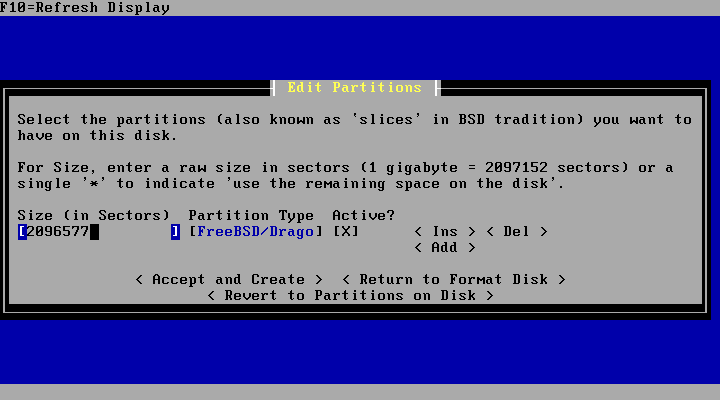
\includegraphics[scale=0.7]{pics/Installer_edit_partitions.eps} \\
%	\end{center}
%\end{figure}
%
%\subsection{Related to Filesystems, Disks, Storage}
%\begin{figure}[hb]
%	\begin{center}
%		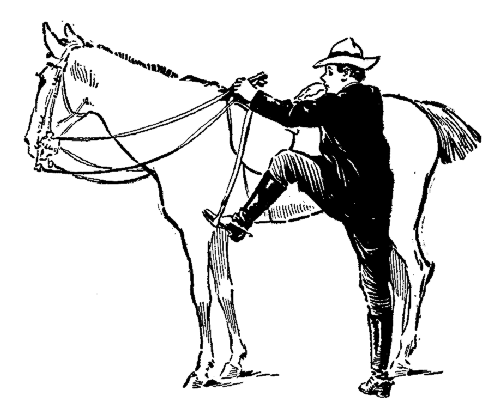
\includegraphics[scale=2.0]{pics/mounting.eps} \\
%	\end{center}
%\end{figure}
%
%\subsection{Related to Filesystems, Disks, Storage}
%\begin{figure}[hb]
%	\begin{center}
%		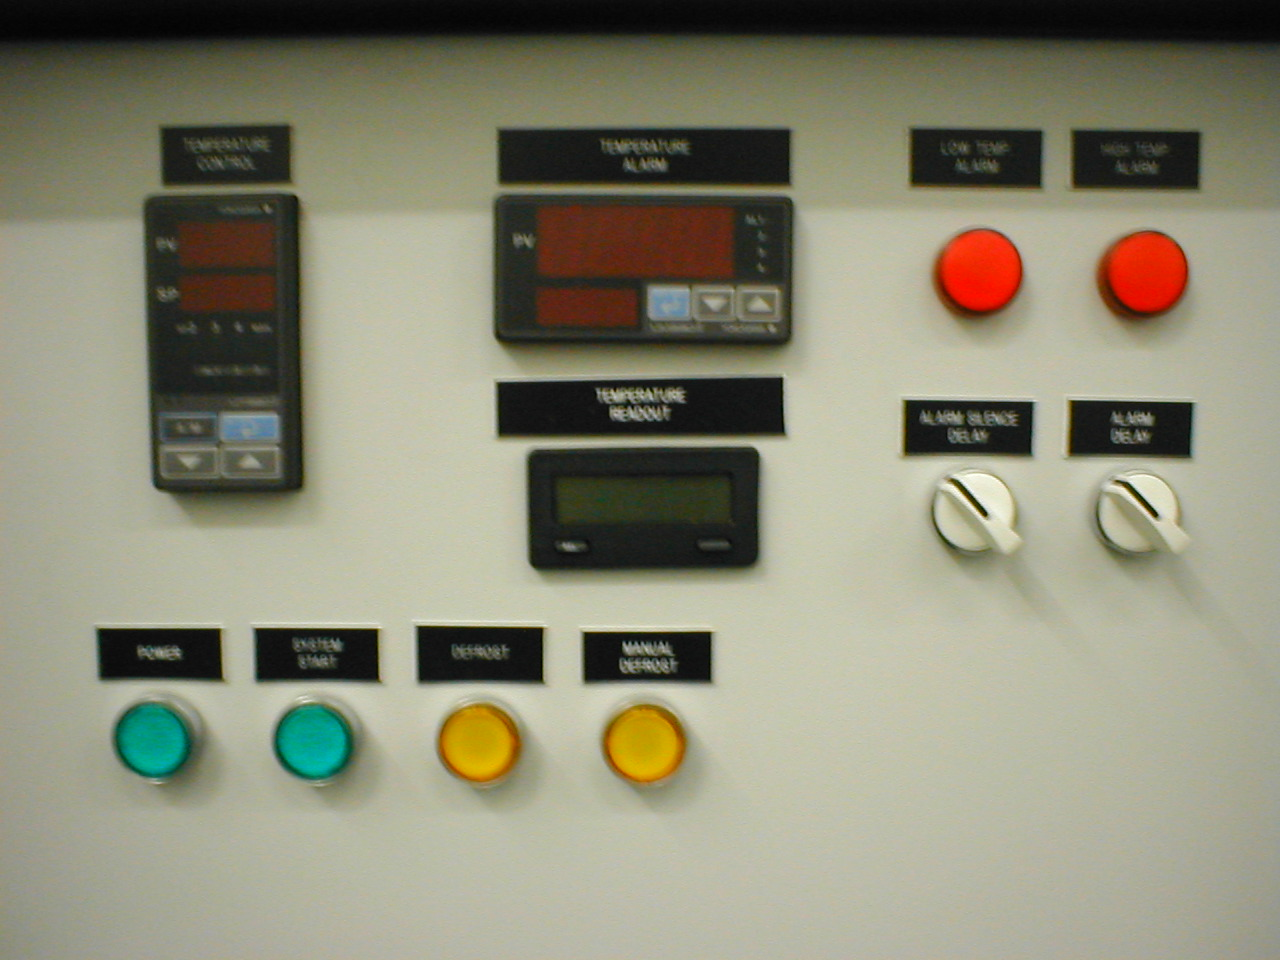
\includegraphics[scale=0.3]{pics/controlpanel.eps} \\
%	\end{center}
%\end{figure}
%
%

\subsection{Topics covered}
Adding, (re-)partitioning, mounting disks requires understanding of:
\begin{itemize}
	\item basic disk concepts
	\item basic filesystem concepts
	\item file systems
\end{itemize}

\subsection{Topics covered}
Adding, (re-)partitioning, mounting disks requires understanding of:
\begin{itemize}
	\item basic disk concepts
		\begin{itemize}
			\item storage models
			\item disk interfaces
			\item physical disk structure
			\item partitions
		\end{itemize}
	\item basic filesystem concepts
	\item file systems
\end{itemize}

\subsection{Topics covered}
Adding, (re-)partitioning, mounting disks requires understanding of:
\begin{itemize}
	\item basic disk concepts
		\begin{itemize}
			\item storage models
			\item disk interfaces
			\item physical disk structure
			\item partitions
		\end{itemize}
	\item basic filesystem concepts
		\begin{itemize}
			\item RAID
			\item logical volume managment
			\item device formatting
		\end{itemize}
	\item file systems
\end{itemize}

\subsection{Topics covered}
Adding, (re-)partitioning, mounting disks requires understanding of:
\begin{itemize}
	\item basic disk concepts
		\begin{itemize}
			\item storage models
			\item disk interfaces
			\item physical disk structure
			\item partitions
		\end{itemize}
	\item basic filesystem concepts
		\begin{itemize}
			\item RAID
			\item logical volume managment
			\item device formatting
		\end{itemize}
	\item file systems
		\begin{itemize}
			\item the UNIX filesystem or Berkeley Fast File System (FFS)
		\end{itemize}
\end{itemize}

\newpage
\vspace*{\fill}
\begin{center}
	\Hugesize
		Basic Disk Concepts \\ [1em]
	\hspace*{5mm}
	\blueline\\
	\hspace*{5mm}\\
		Storage Models
\end{center}
\vspace*{\fill}

\subsection{Basic Disk Concepts: Storage Models}
Direct Attached Storage (DAS)
\vfill
\begin{center}
	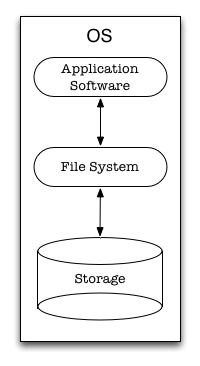
\includegraphics[scale=0.8]{pics/das.eps} \\
\end{center}
\vfill

\subsection{Basic Disk Concepts: Storage Models}
Network Attached Storage (NAS)
\vfill
\begin{center}
	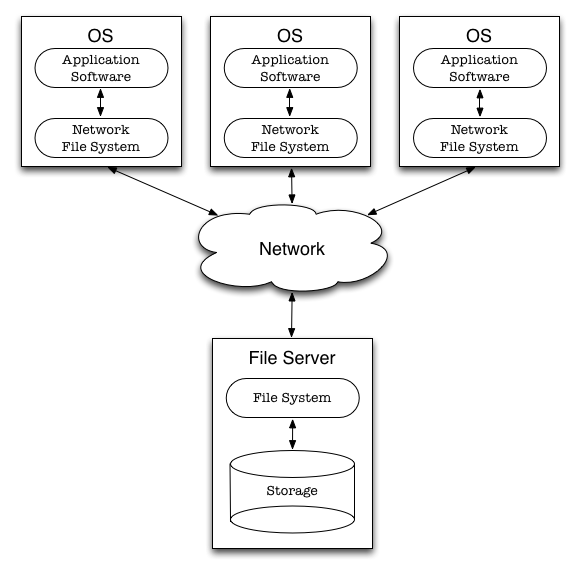
\includegraphics[scale=0.5]{pics/nas.eps} \\
\end{center}
\vfill

\subsection{Basic Disk Concepts: Storage Models}
Storage Area Networks (SAN)
\vfill
\begin{center}
	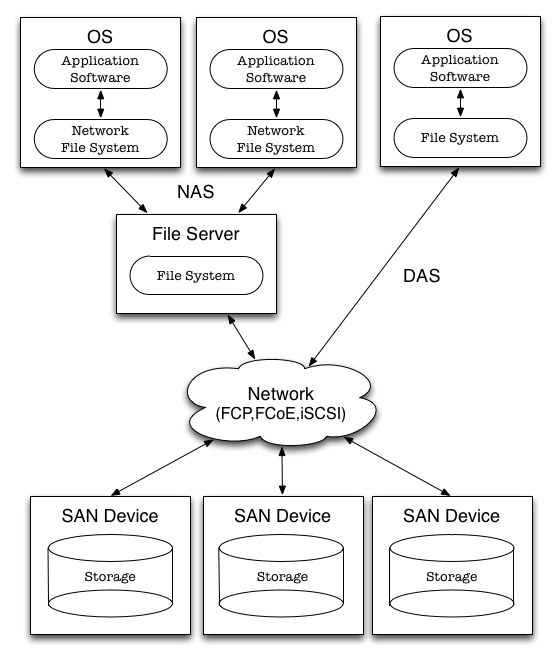
\includegraphics[scale=0.5]{pics/san-nas-das.eps} \\
\end{center}
\vfill

\subsection{Basic Disk Concepts: Storage Models}
Cloud Storage (Examples: EBS, S3)
\vfill
\begin{center}
	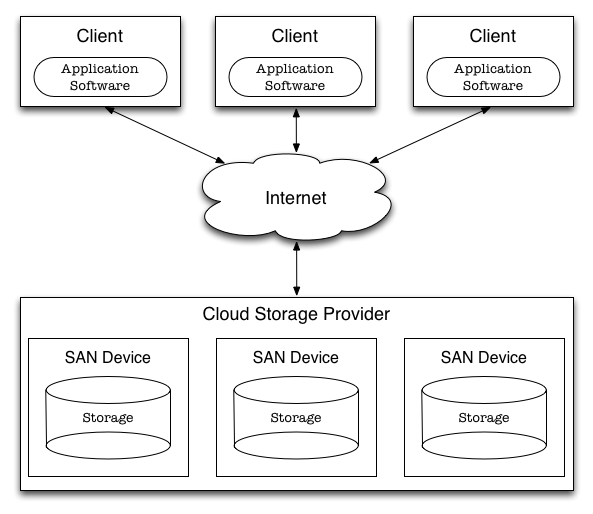
\includegraphics[scale=0.6]{pics/cloud-storage.eps} \\
\end{center}
\vfill

\newpage
\vspace*{\fill}
\begin{center}
	\Hugesize
		Basic Disk Concepts \\ [1em]
	\hspace*{5mm}
	\blueline\\
	\hspace*{5mm}\\
		Disk Devices
\end{center}
\vspace*{\fill}


\subsection{Basic Disk Concepts: Disk Devices}
	\begin{center}
		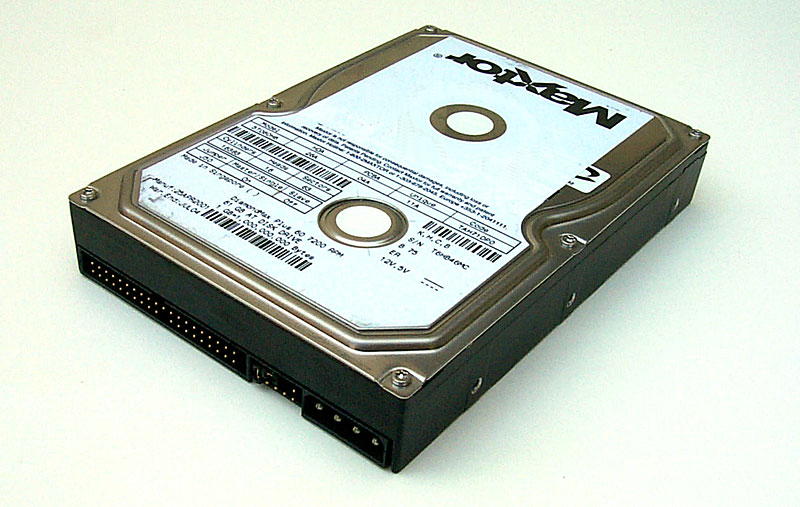
\includegraphics[scale=0.9]{pics/ide-drive.eps} \\
	\end{center}

\subsection{Basic Disk Concepts: Disk Devices}
	\begin{center}
		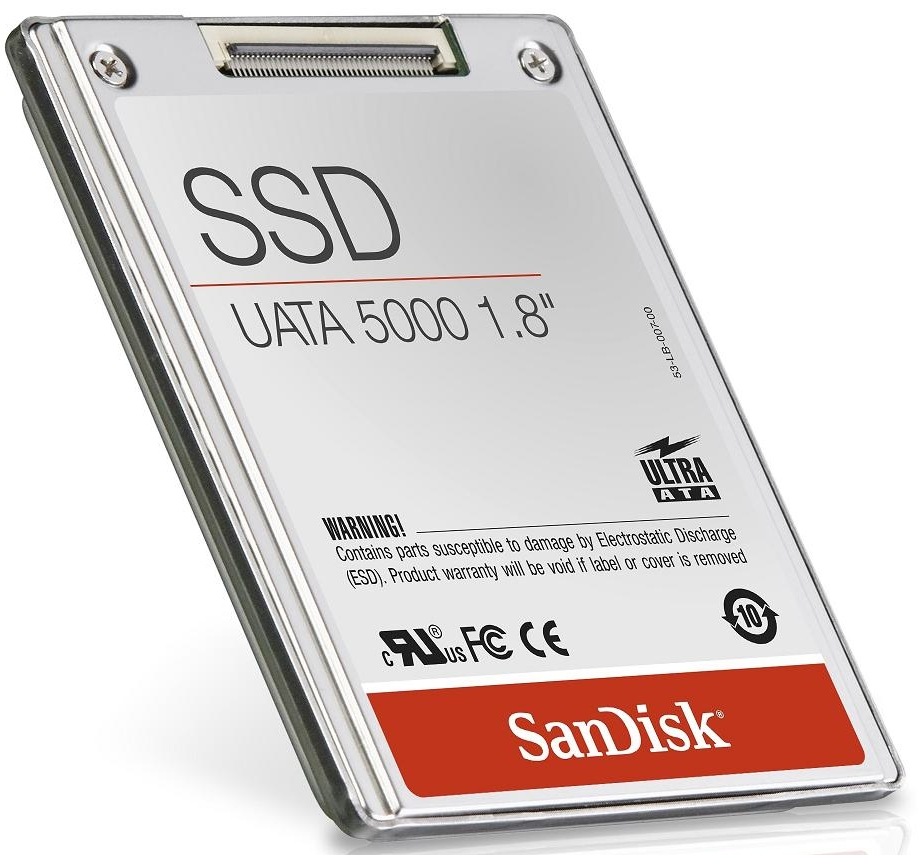
\includegraphics[scale=0.5]{pics/ssd.eps} \\
	\end{center}

\subsection{Basic Disk Concepts: Disk Devices}
	\begin{center}
		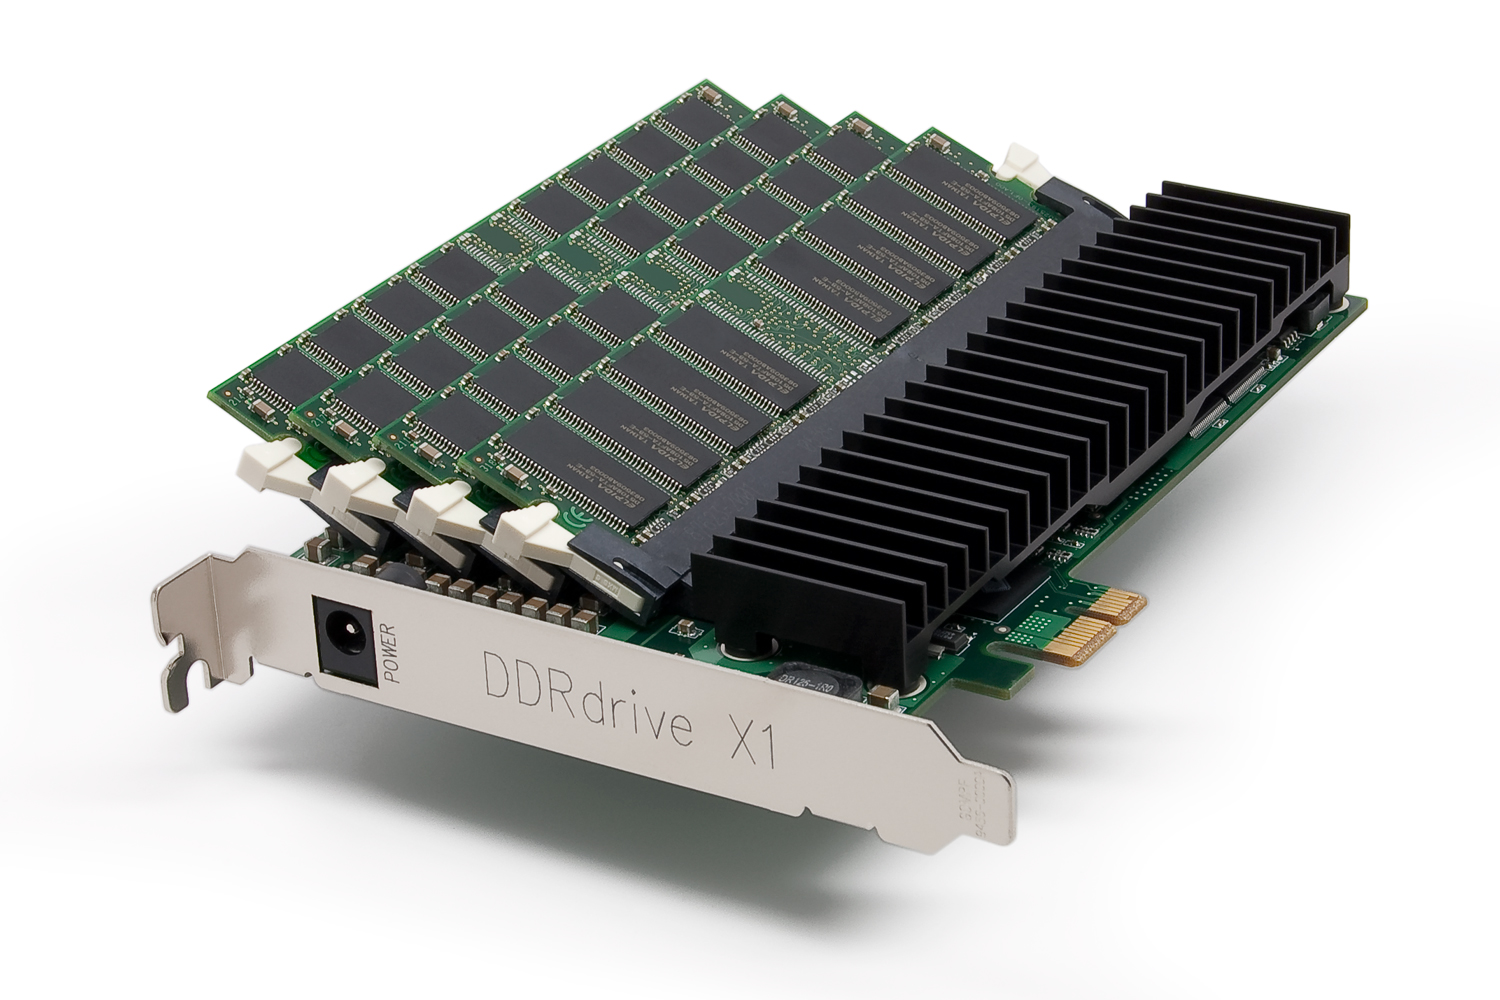
\includegraphics[scale=0.5]{pics/ddrdrive.eps} \\
	\end{center}

\subsection{Basic Disk Concepts: Disk Devices}
\begin{figure}[hb]
	\begin{center}
		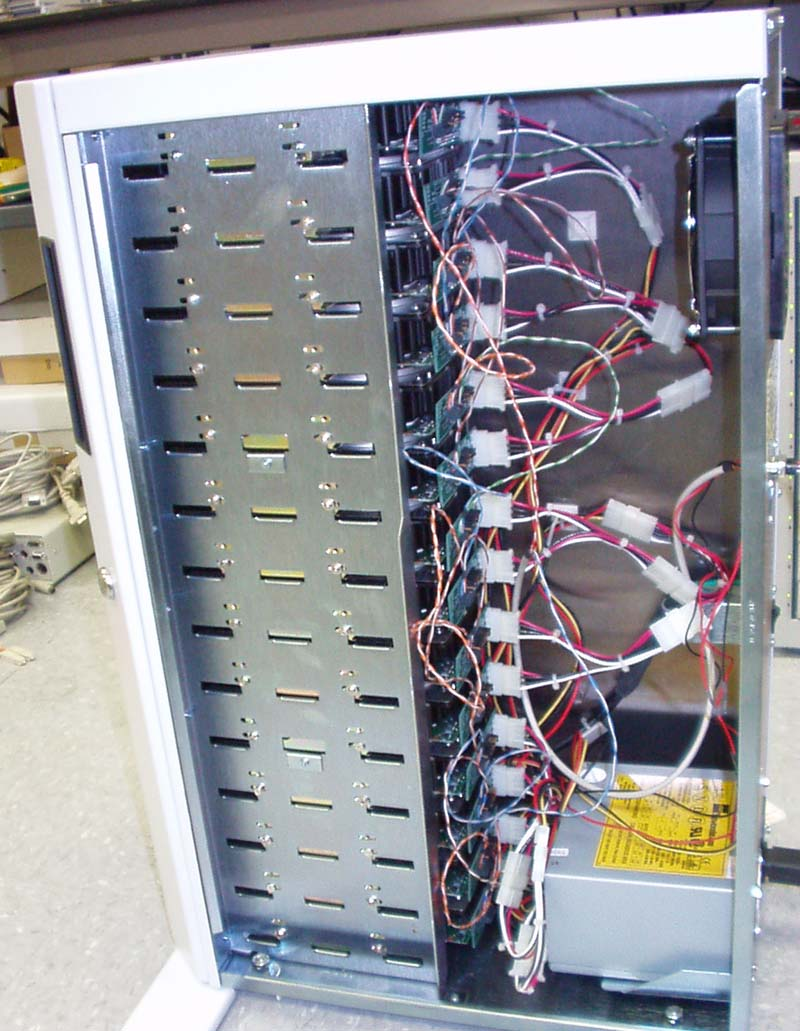
\includegraphics[scale=0.5]{pics/jbod-inside.eps}
		\hspace*{15mm}
		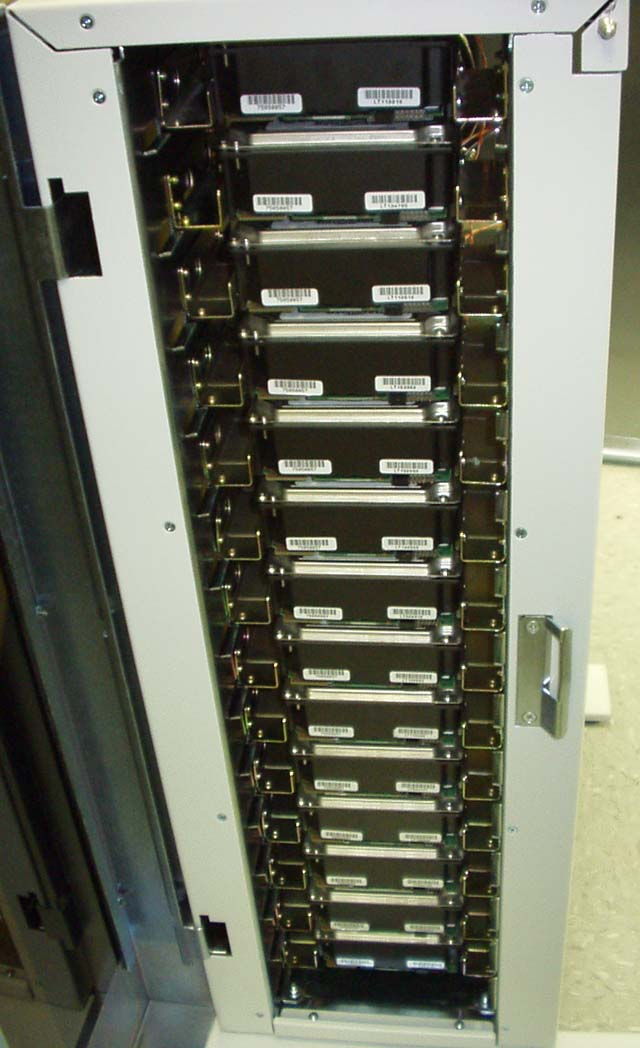
\includegraphics[scale=0.5]{pics/jbod-front.eps} \\
	\end{center}
\end{figure}


\subsection{Basic Disk Concepts: Disk Devices}
\vfill
	\begin{center}
		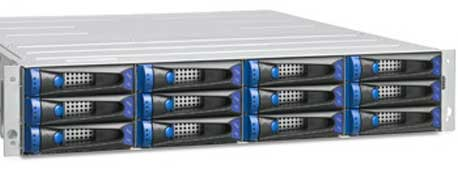
\includegraphics[scale=1.5]{pics/S50JBOD.eps} \\
	\end{center}
\vfill

\subsection{Basic Disk Concepts: Disk Devices}
	\begin{center}
		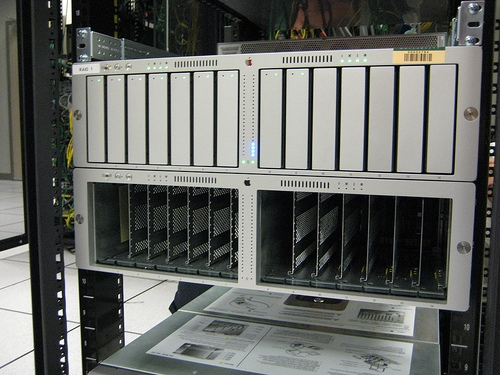
\includegraphics[scale=0.9]{pics/xraid.eps} \\
	\end{center}


\subsection{Basic Disk Concepts: Disk Devices}
	\begin{center}
		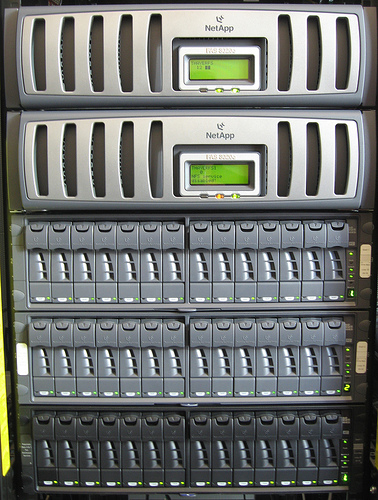
\includegraphics[scale=0.7]{pics/netapp.eps} \\
	\end{center}

\newpage
\vspace*{\fill}
\begin{center}
	\Hugesize
		Basic Disk Concepts \\ [1em]
	\hspace*{5mm}
	\blueline\\
	\hspace*{5mm}\\
		Disk Interfaces
\end{center}
\vspace*{\fill}

\subsection{Basic Disk Concepts: Disk Interfaces: SCSI}
	\begin{center}
		\includegraphics[scale=0.8]{pics/scsi-many.eps} \\
	\end{center}


\subsection{Basic Disk Concepts: Disk Interfaces: SCSI}
\begin{figure}[hb]
	\begin{center}
		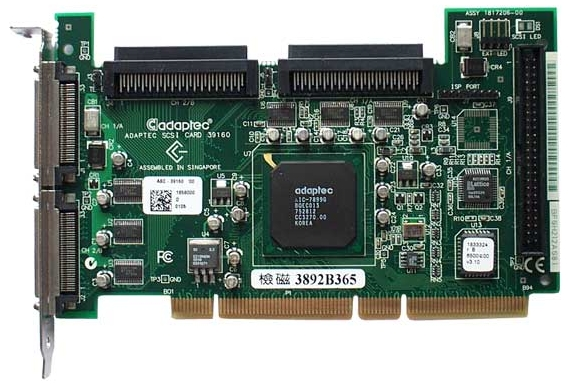
\includegraphics[scale=0.7]{pics/scsicard.eps} \\
	\end{center}
\end{figure}

\subsection{Basic Disk Concepts: Disk Interfaces: SCSI}
\vfill
	\begin{center}
		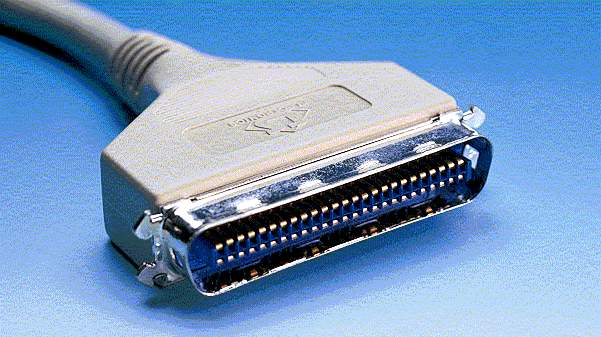
\includegraphics[scale=0.8]{pics/cable_scsi.eps} \\
	\end{center}
\vfill

%\subsection{Basic Disk Concepts: Disk Interfaces: SCSI}
%\begin{figure}[hb]
%	\begin{center}
%		\includegraphics[scale=1.0]{pics/scsi-types.eps} \\
%	\end{center}
%\end{figure}

\subsection{Basic Disk Concepts: Disk Interfaces: SCSI}
\vfill
	\begin{center}
		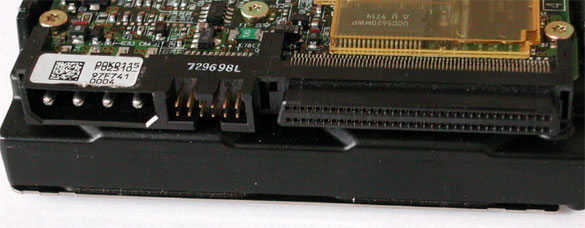
\includegraphics[scale=1.0]{pics/scsi-disk.eps} \\
	\end{center}
\vfill

%\subsection{Basic Disk Concepts: Disk Interfaces: SCSI}
%\begin{figure}[hb]
%	\begin{center}
%		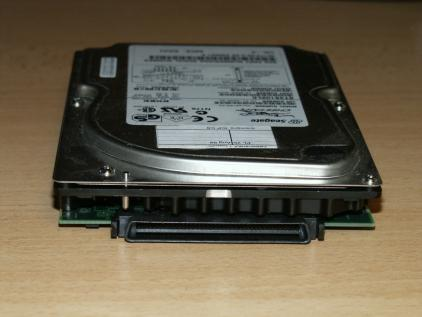
\includegraphics[scale=0.9]{pics/scsi-disk2.eps} \\
%	\end{center}
%\end{figure}

\subsection{Basic Disk Concepts: Disk Interfaces: SCSI}
\vfill
	\begin{center}
		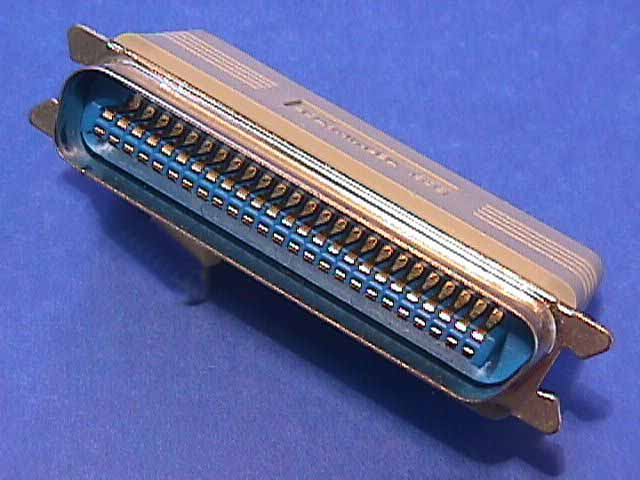
\includegraphics[scale=0.7]{pics/scsi-terminator.eps} \\
	\end{center}
\vfill

\subsection{Basic Disk Concepts: Disk Interfaces: SCSI}
Too many variations (Fast, Wide, Ultra, ...).
\begin{itemize}
	\item each SCSI device needs a terminator (internal or terminator plug)
	\item each SCSI device (including the controller) needs a target number
		(or ID)
	\item this ID needs to be {\em unique}
	\item a single slower/older device will bring down speed for {\em all}
		devices attached to that controller
	\item hot swappable
	\item speed: up to 640 MB/s
	\item max cable length: up to 16 m
	\item max number of devices: up to 16
\end{itemize}

% IDE
\subsection{Basic Disk Concepts: Disk Interfaces: ATA}
\vfill
	\begin{center}
		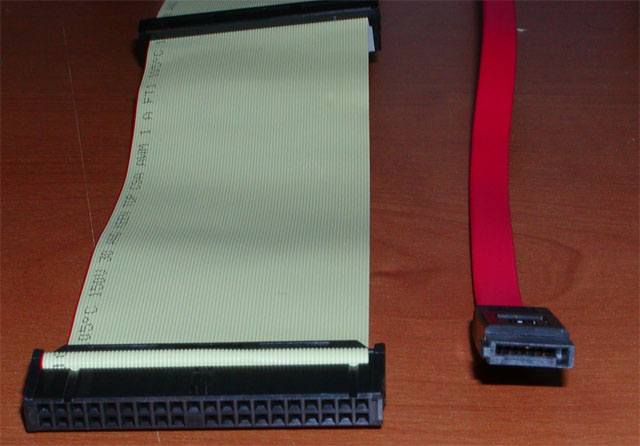
\includegraphics[scale=0.8]{pics/satavpata.eps} \\
	\end{center}
\vfill

\subsection{Basic Disk Concepts: Disk Interfaces: ATA}
\vfill
	\begin{center}
		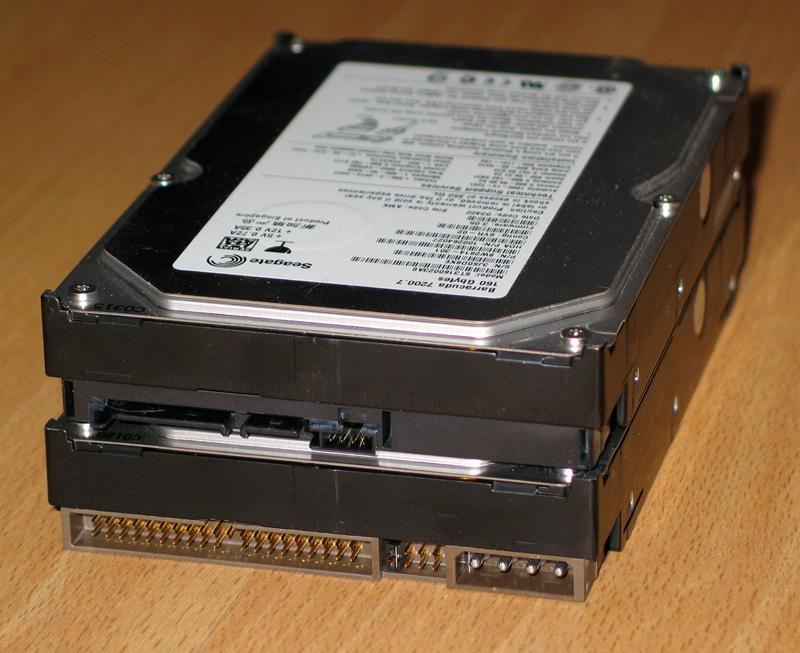
\includegraphics[scale=1.1]{pics/satavide.eps} \\
	\end{center}
\vfill

\subsection{Basic Disk Concepts: Disk Interfaces: ATA}
\vfill
	\begin{center}
		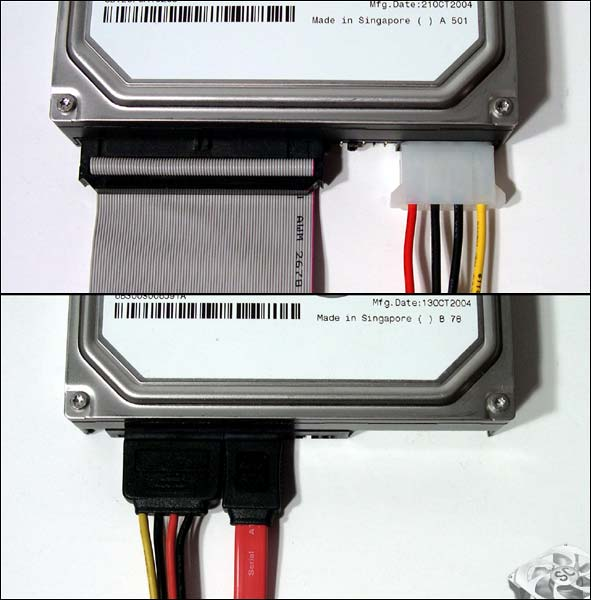
\includegraphics[scale=0.75]{pics/sata-ide_lg.eps} \\
	\end{center}
\vfill


\subsection{Basic Disk Concepts: Disk Interfaces: ATA}
``Advanced Technology Attachment''
\begin{itemize}
	\item Parallel ATA:
	\begin{itemize}
		\item Enhanced Integrated Device Electronics (EIDE)
		\item Extensions known as Advanced Technology Attachment Packet
			Interface (ATAPI)
		\item designed to be simple and inexpensive (controller build
			into the disk)
		\item speed: up to 133 MB/s; max cable length: up to 46cm; number of devices: 2
	\end{itemize}
	\item Serial ATA:
	\begin{itemize}
		\item hot-pluggable
		\item speed: up to 6 Gb/s (``SATA Revision 3''); up to 1.5 Gb/s (``SATA Revision 1.0'')
		\item max cable length: 1 m up to 2 m (``eSATA'')
		\item number of devices: 1
	\end{itemize}
\end{itemize}

\subsection{Basic Disk Concepts: Disk Interfaces: SATA}
%\begin{figure}[hb]
	\begin{center}
		\includegraphics[scale=0.77]{pics/Sata_host_expansor_en.eps} \\
	\end{center}
%\end{figure}

% USB

\subsection{Basic Disk Concepts: Disk Interfaces: USB}
\vfill
	\begin{center}
		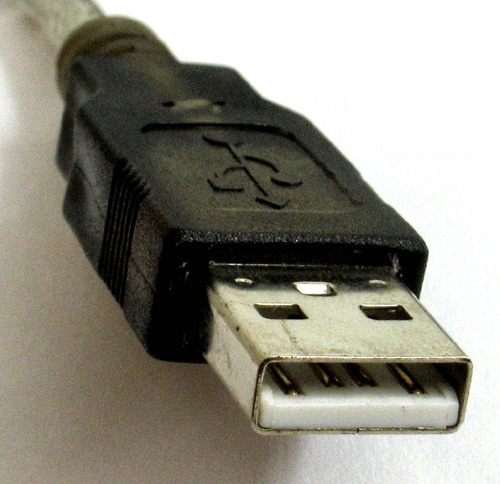
\includegraphics[scale=0.8]{pics/USB_Connector_End.eps} \\
	\end{center}
\vfill

\subsection{Basic Disk Concepts: Disk Interfaces: USB}
\vfill
	\begin{center}
		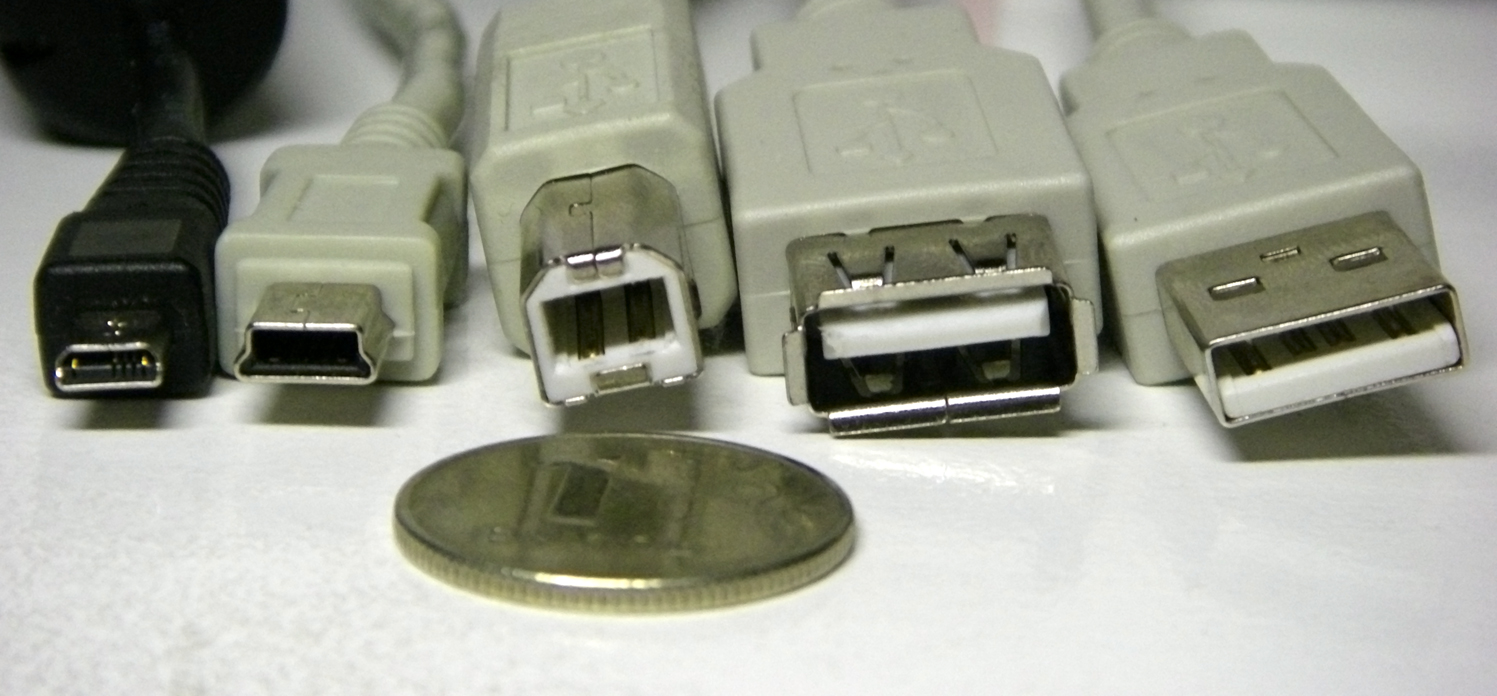
\includegraphics[scale=0.6]{pics/USB_types.eps} \\
	\end{center}
\vfill

\subsection{Basic Disk Concepts: Disk Interfaces: USB}
\vfill
	\begin{center}
		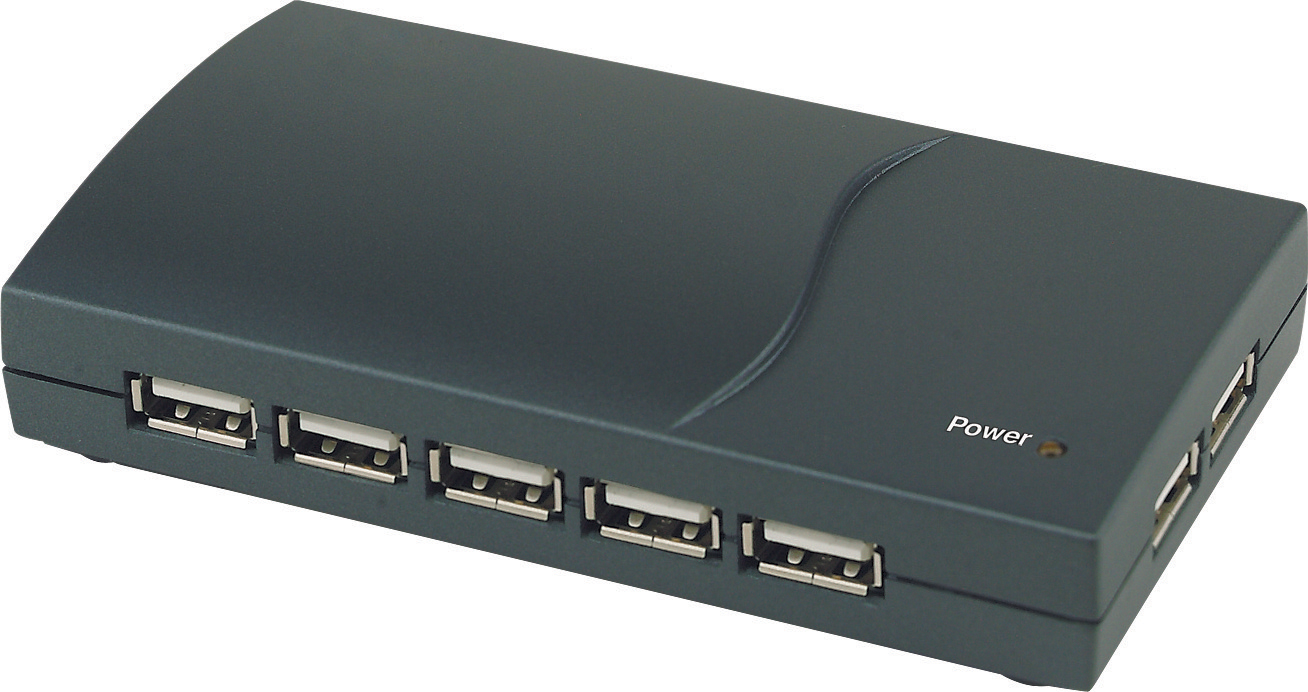
\includegraphics[scale=0.6]{pics/usb-hub.eps} \\
	\end{center}
\vfill

\subsection{Basic Disk Concepts: Disk Interfaces: USB}
``Universal Serial Bus''
\begin{itemize}
	\item can provide power
	\item hot-pluggable
	\item (theoretical) speed: 12 Mb/s in USB 1.0; up to 480 Mb/s in USB 2.0; up to 4 Gb/s in USB 3.0
	\item max cable length: up to 5 m
	\item number of devices: up to 127
\end{itemize}


% FW

\subsection{Basic Disk Concepts: Disk Interfaces: FireWire}
\vfill
	\begin{center}
		
\includegraphics[scale=0.4]{pics/fw.eps} \\
	\end{center}
\vfill


\subsection{Basic Disk Concepts: Disk Interfaces: FireWire}
\vfill
	\begin{center}
		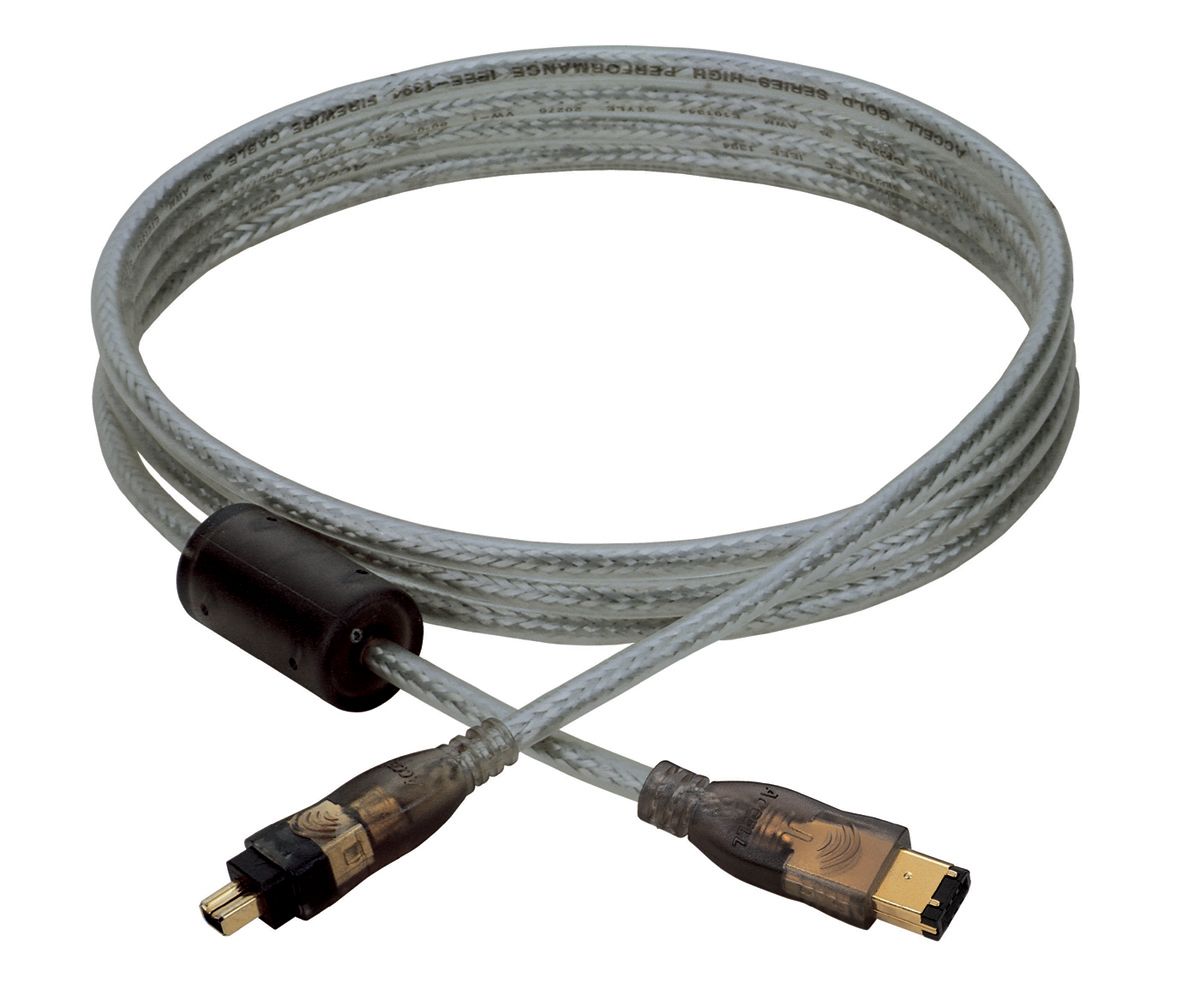
\includegraphics[scale=1.2]{pics/FireWire_4_6Pin.eps} \\
	\end{center}
\vfill

\subsection{Basic Disk Concepts: Disk Interfaces: FireWire}
\vfill
	\begin{center}
		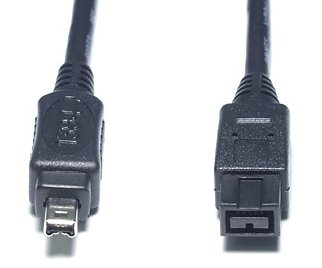
\includegraphics[scale=2.4]{pics/fw1.eps}
		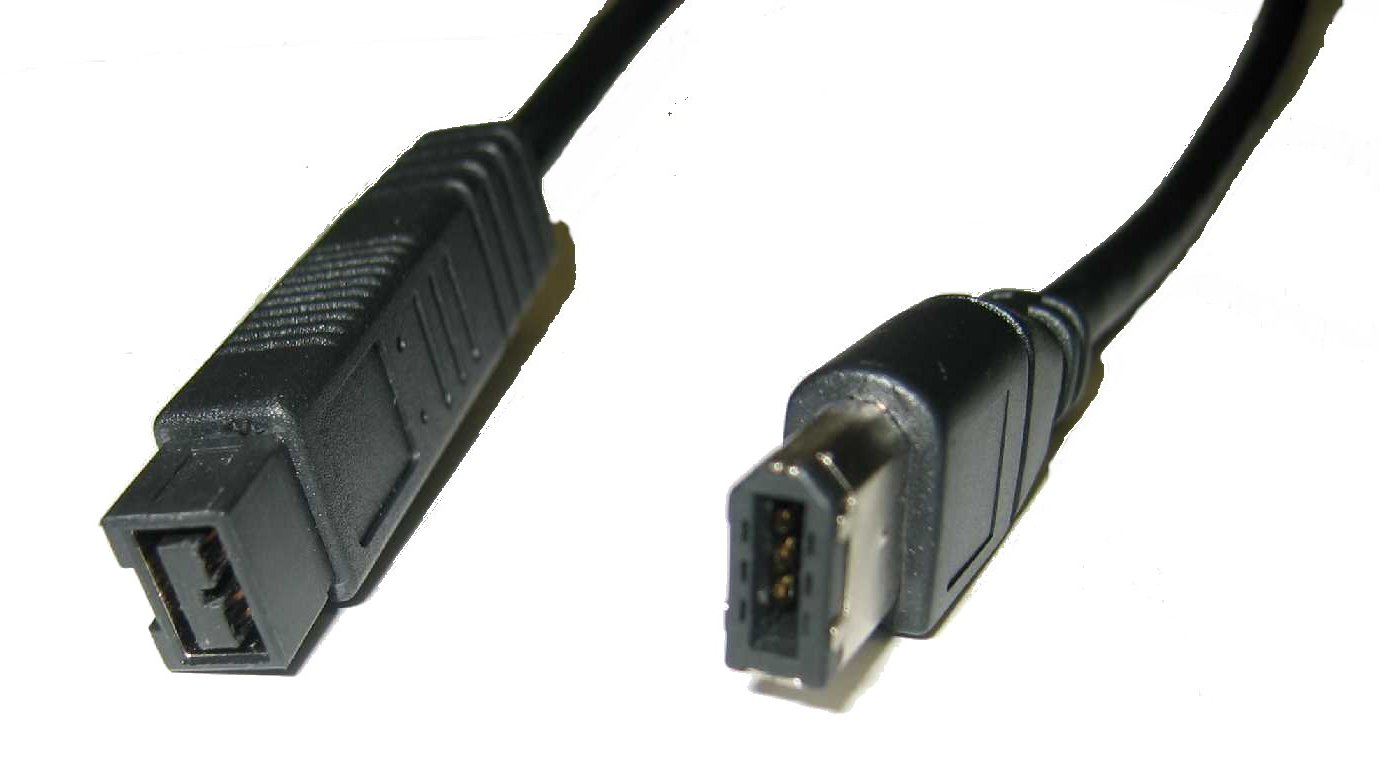
\includegraphics[scale=0.8]{pics/fw2.eps}
		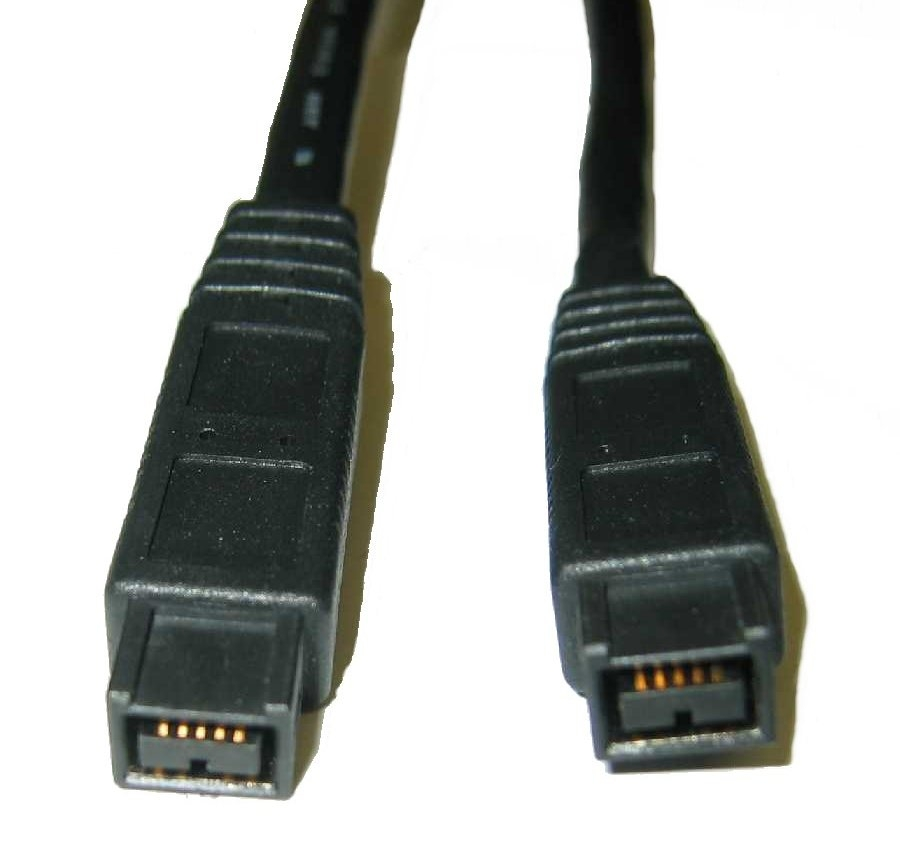
\includegraphics[scale=0.8]{pics/fw3.eps}
	\end{center}
\vfill

\subsection{Basic Disk Concepts: Disk Interfaces: FireWire}
FireWire, aka IEEE 1394
\begin{itemize}
	\item speed: 400 Mb/s, 800 Mb/s and even up to 3.2 Gbit/s
	\item hot-pluggable
	\item max cable length: up to 100 m
	\item number of devices: up to 63
\end{itemize}
\newpage

% FC

\subsection{Basic Disk Concepts: Disk Interfaces: Fibre Channel}
\vfill
	\begin{center}
		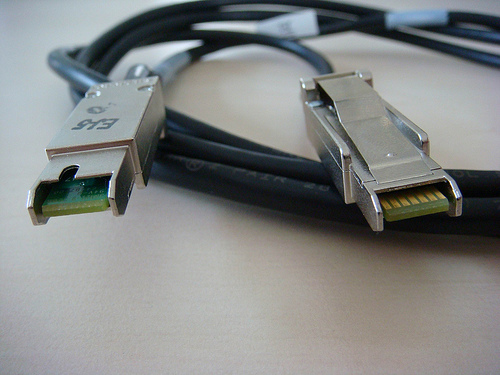
\includegraphics[scale=0.9]{pics/fc-connector.eps} \\
	\end{center}
\vfill

\subsection{Basic Disk Concepts: Disk Interfaces: Fibre Channel}
\vfill
	\begin{center}
		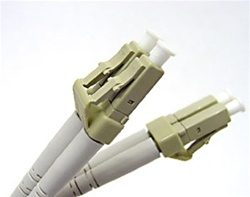
\includegraphics[scale=1.5]{pics/fc-optical.eps} \\
	\end{center}
\vfill

\subsection{Basic Disk Concepts: Disk Interfaces: Fibre Channel}
\vfill
	\begin{center}
		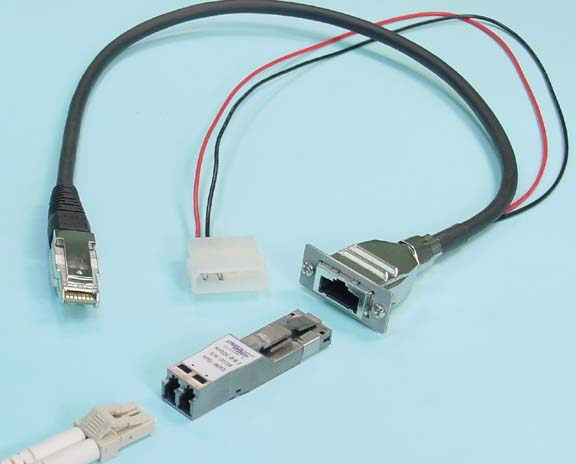
\includegraphics[scale=0.7]{pics/fc-connectors.eps} \\
	\end{center}
\vfill

\subsection{Basic Disk Concepts: Disk Interfaces: Fibre Channel}
\vfill
	\begin{center}
		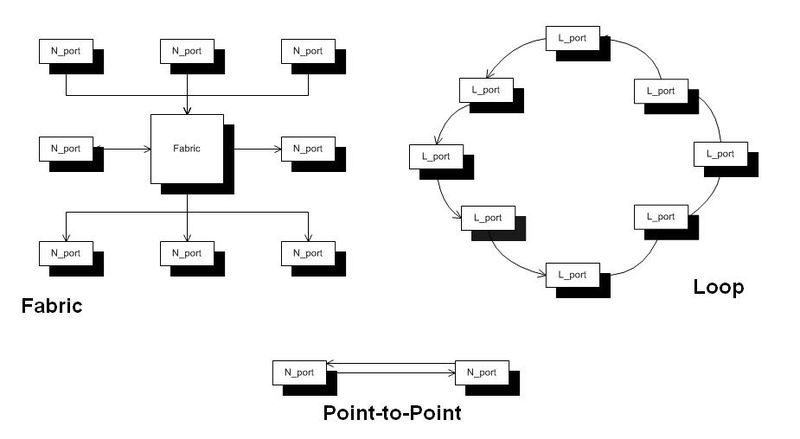
\includegraphics[scale=1.0]{pics/fc-topologies.eps} \\
	\end{center}
\vfill

\subsection{Basic Disk Concepts: Disk Interfaces: Fibre Channel}
\vfill
	\begin{center}
		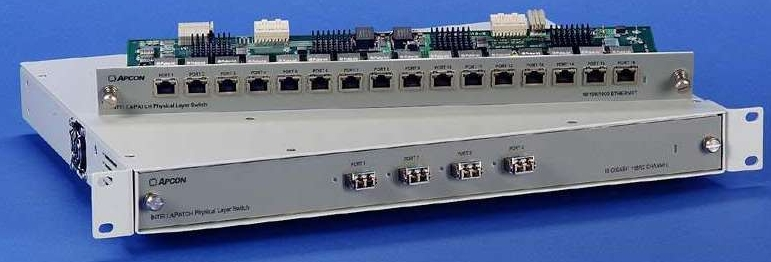
\includegraphics[scale=0.8]{pics/fc-switch.eps} \\
	\end{center}
\vfill

\subsection{Basic Disk Concepts: Disk Interfaces: Fibre Channel}
\vfill
	\begin{center}
		\includegraphics[scale=0.4]{pics/fc-switched.eps} \\
	\end{center}
\vfill

\subsection{Basic Disk Concepts: Disk Interfaces: Fibre Channel}
Fibre Channel:
\begin{itemize}
	\item point-to-point,in arbitrated loop or switched
	\item hot-pluggable
	\item speeds: up to 16  Gb/s
	\item max cable length: up to 20 m (copper) or up to 50 km (Optical)
	\item number of devices: 2 (point-to-point), 127 (loop), or... $2^{24}$ (switched)
\end{itemize}

% SAS - Serial Attached SCSI
\subsection{Basic Disk Concepts: Disk Interfaces: SAS}
Serial Attached SCSI
\vfill
\begin{center}
	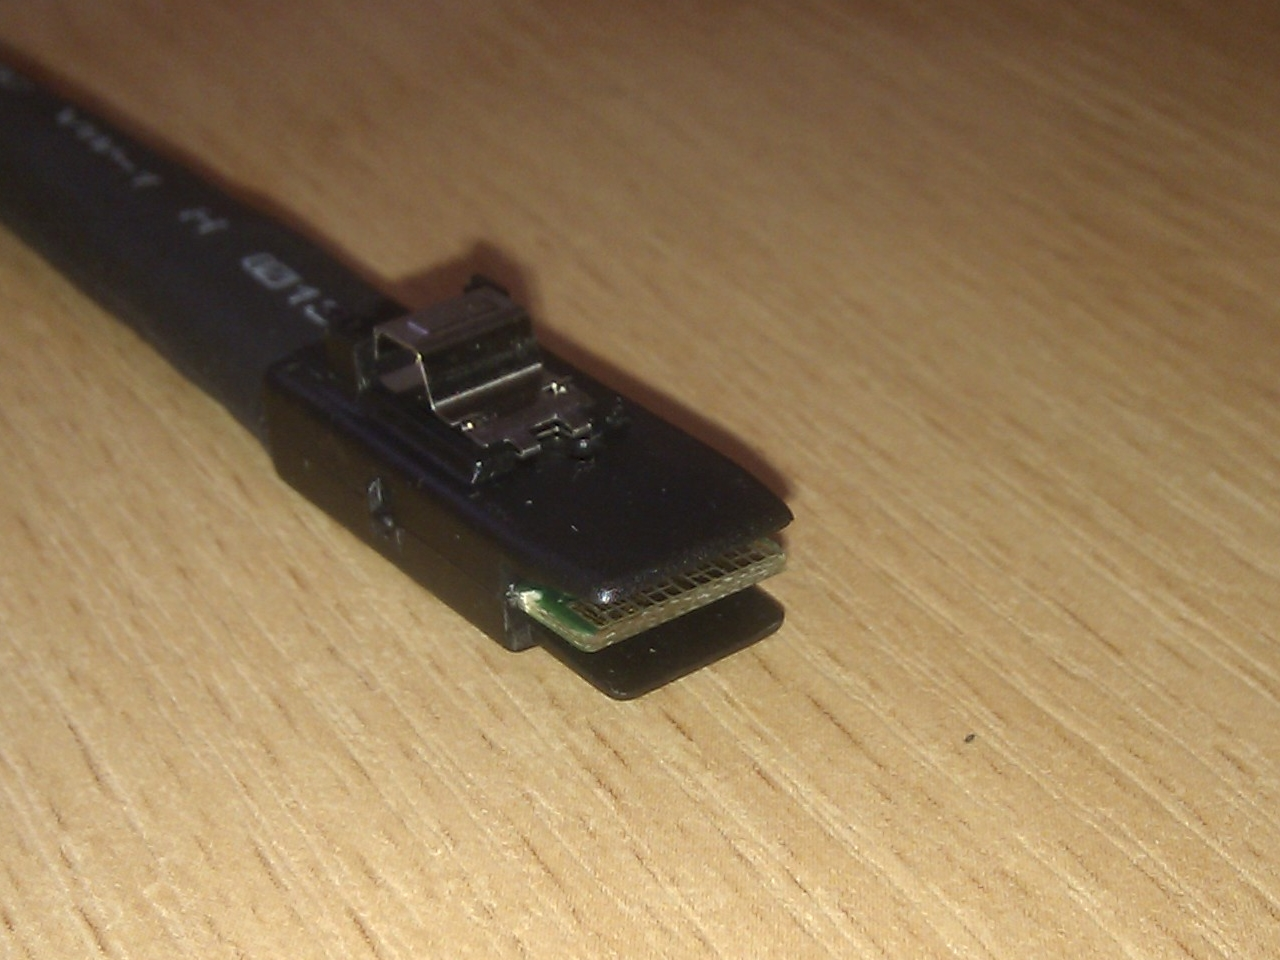
\includegraphics[scale=0.1]{pics/SFF_8086.eps}
	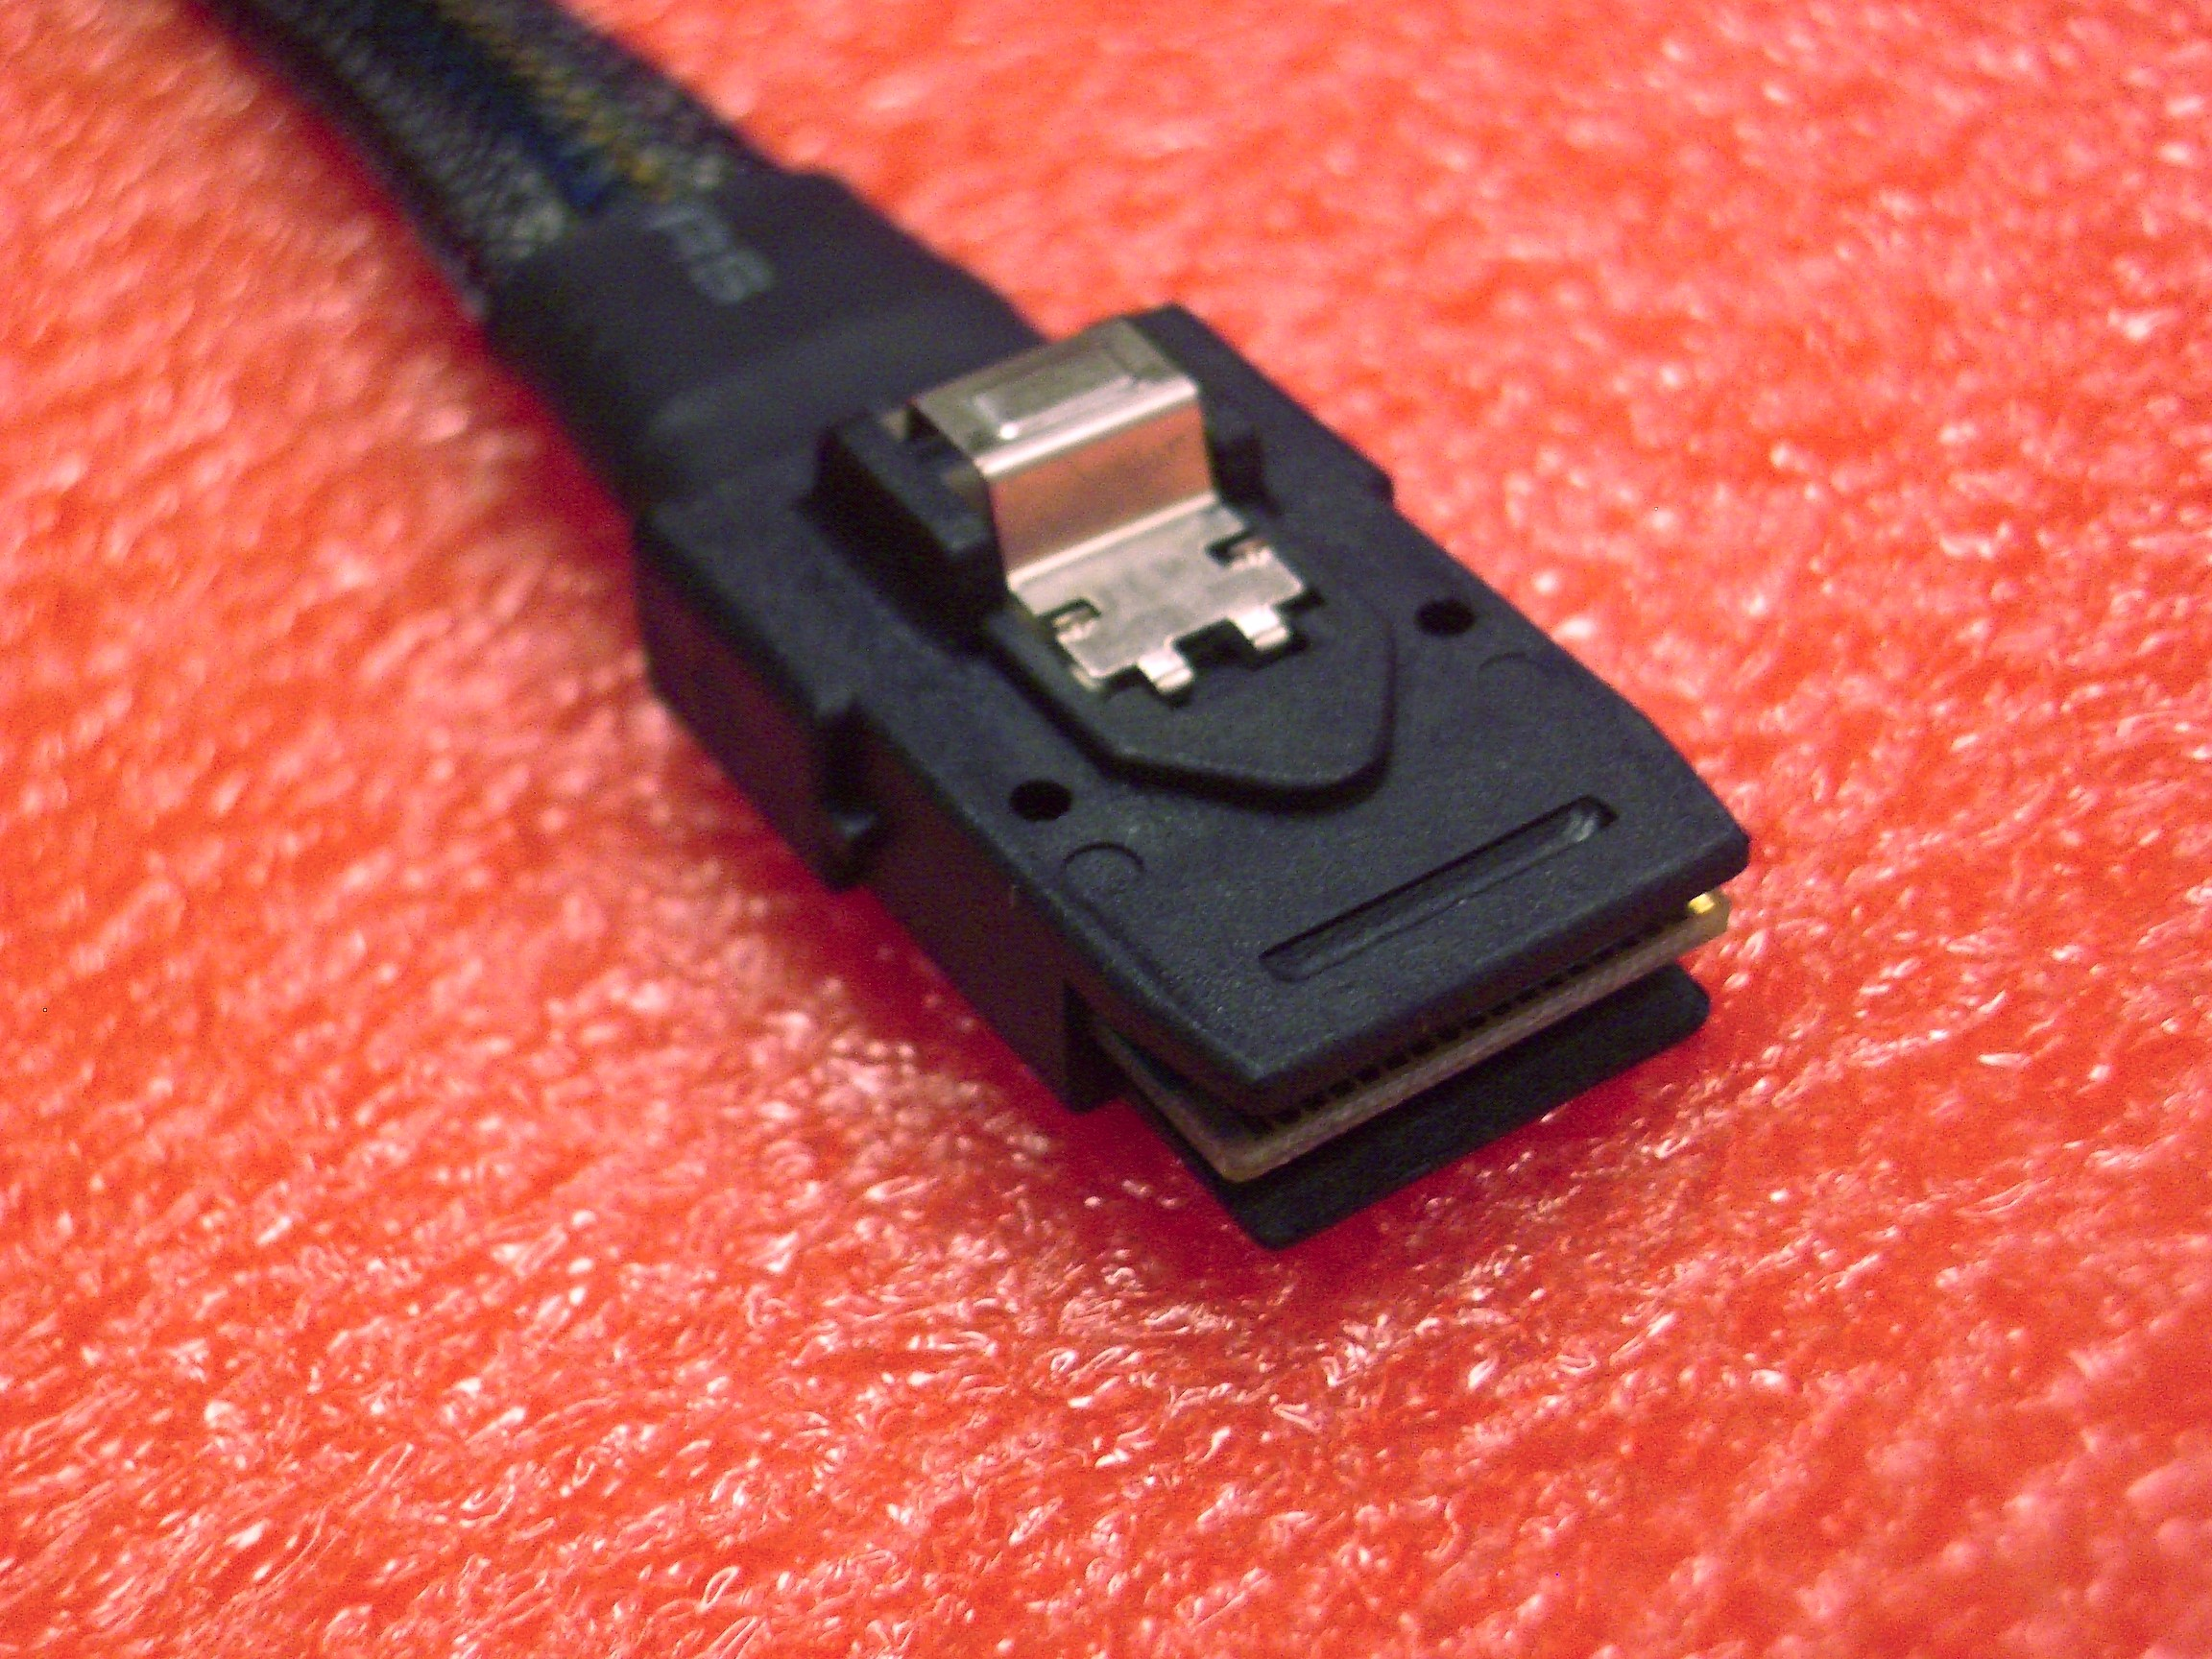
\includegraphics[scale=0.07]{pics/SFF_8087.eps}
	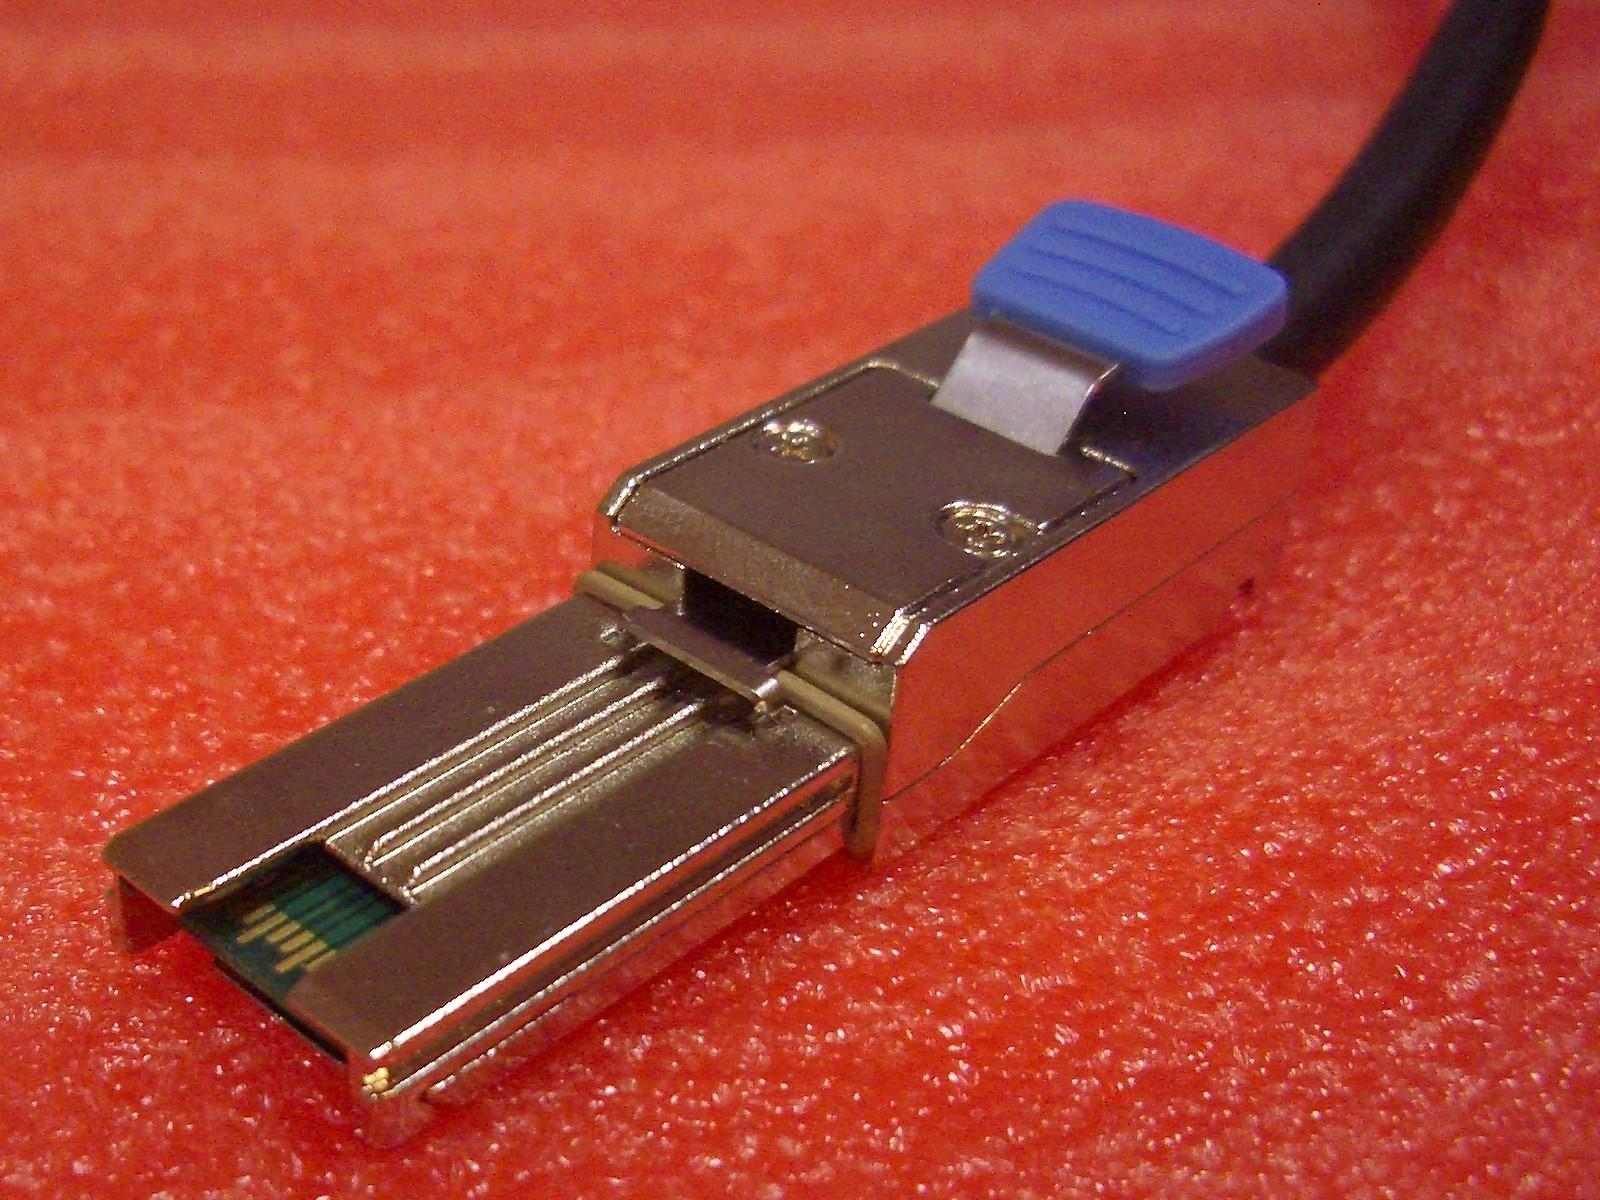
\includegraphics[scale=0.1]{pics/SFF_8088.eps}
	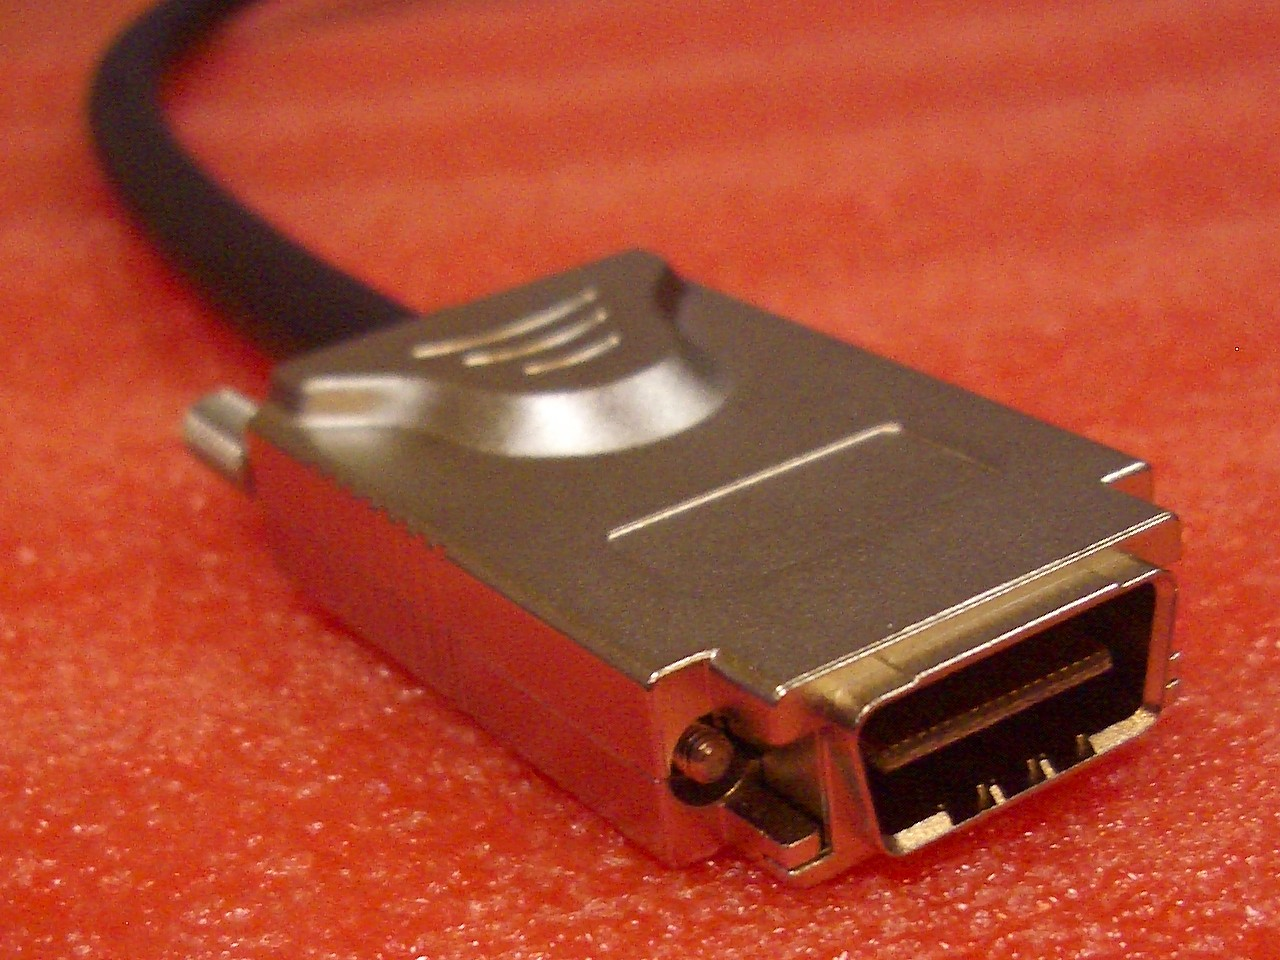
\includegraphics[scale=0.1]{pics/SFF_8470.eps}
	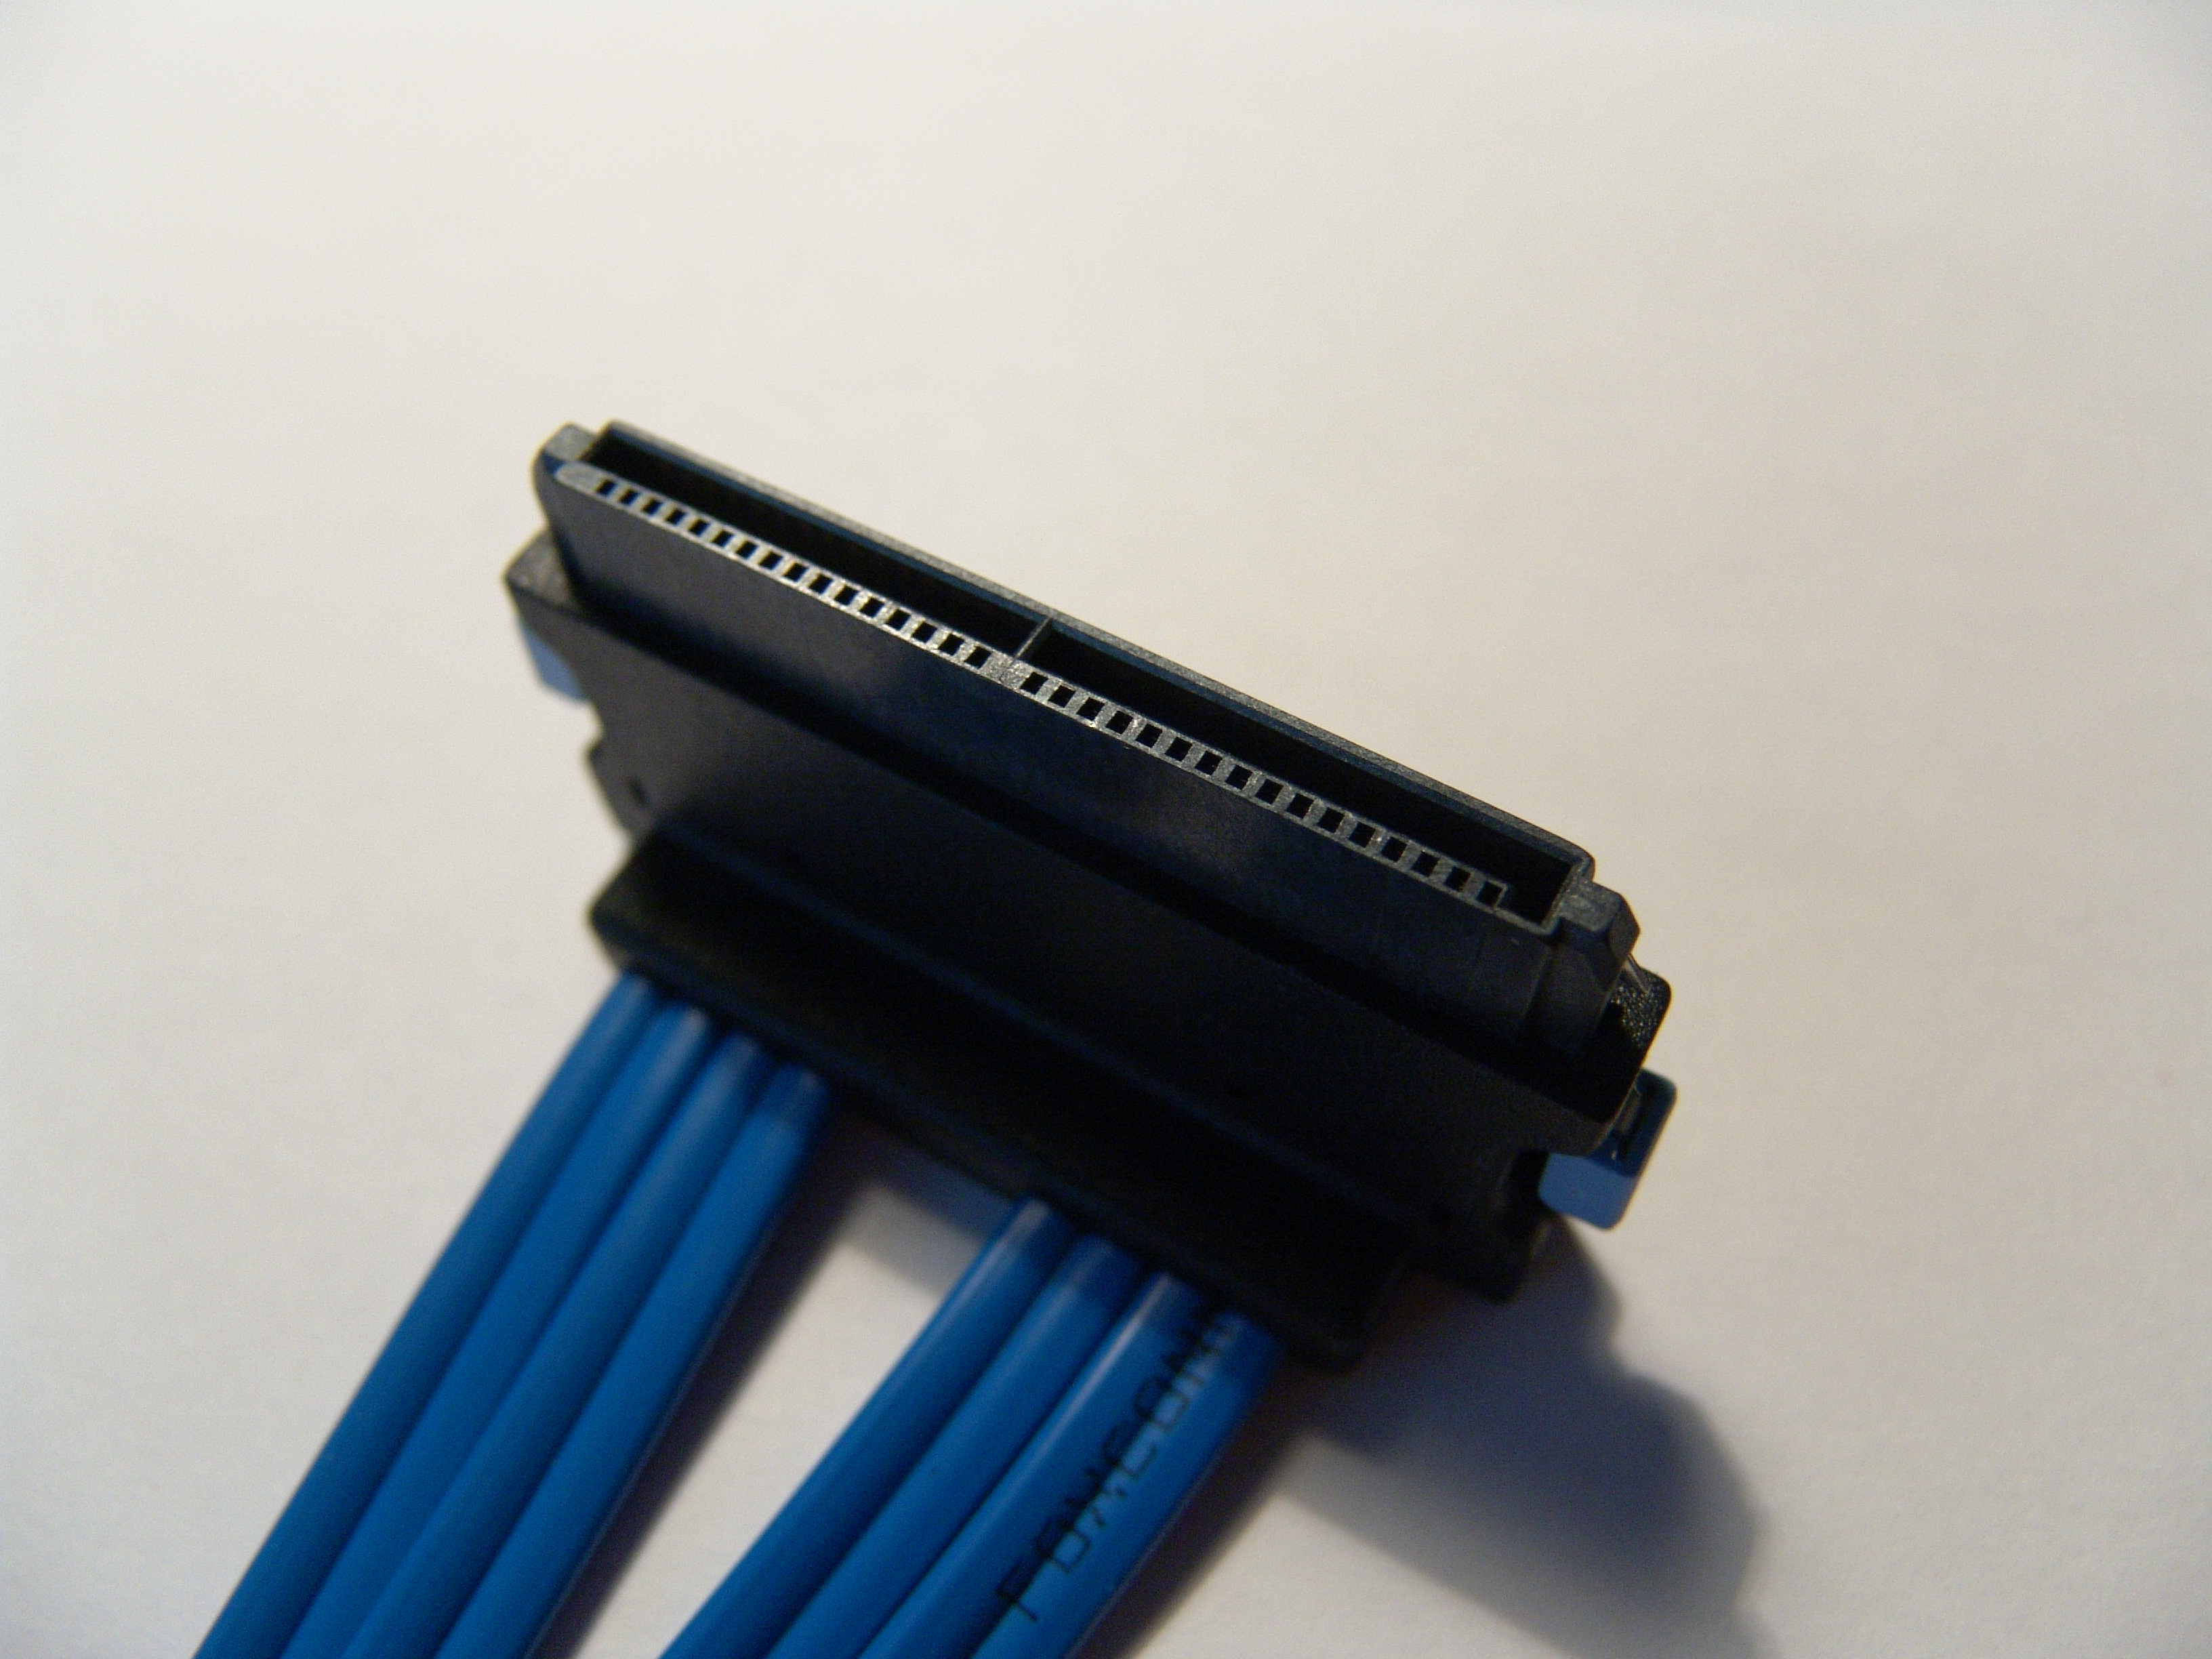
\includegraphics[scale=0.05]{pics/SFF_8484_angled.eps}
\end{center}
\vfill

\subsection{Basic Disk Concepts: Disk Interfaces: SAS}
Serial Attached SCSI
\begin{itemize}
	\item point-to-point, but layered model (physical, PHY, link,
		port, transport, application)
	\item transport via SCSI-, SATA-, or fabric managing protocols
	\item backwards compatible with SATA
	\item transfer speeds of up to 6Gb/s; up to $2^{16}$ devices
	\item expanders allow for switched topologies
\end{itemize}



% AoE (ATA over Ethernet)

\subsection{Basic Disk Concepts: Disk Interfaces: SANs}
\begin{itemize}
	\item ATA over Ethernet ({\em AoE}):
		\begin{itemize}
			\item create low-cost SAN
			\item ATA encapsulated into Ethernet frames
		\end{itemize}
	\item Fibre Channel over Ethernet ({\em FCoE}):
		\begin{itemize}
			\item consolidate IP and FC/SAN networks
			\item reduce interface cards in servers
			\item reduce additional cabling and associated costs
			\item FC encapsulated into Ethernet frames
		\end{itemize}
\end{itemize}

\subsection{Basic Disk Concepts: Disk Interfaces: SANs}
\begin{itemize}
	\item ATA over Ethernet ({\em AoE}):
		\begin{itemize}
			\item create low-cost SAN
			\item ATA encapsulated into Ethernet frames
		\end{itemize}
	\item Fibre Channel over Ethernet ({\em FCoE}):
		\begin{itemize}
			\item consolidate IP and FC/SAN networks
			\item reduce interface cards in servers
			\item reduce additional cabling and associated costs
			\item FC encapsulated into Ethernet frames
		\end{itemize}

	\item *oE:
		\begin{itemize}
			\item no TCP/IP overhead
			\item restricted to a single Layer 2 network
			\item no inherent security features
		\end{itemize}
\end{itemize}

% iSCSI
\subsection{Basic Disk Concepts: Disk Interfaces: SANs}
\vfill
\begin{center}
	\includegraphics[scale=0.8]{pics/iscsi-host-bus.eps} \\
\end{center}
\vfill

\subsection{Basic Disk Concepts: Disk Interfaces: SANs}
Internet Small Computer System Interface {\em iSCSI}:
\begin{itemize}
	\item SCSI encapsulated in TCP/IP packets
	\item runs over regular network cables
	\item security:
		\begin{itemize}
			\item uses Challenge-handshake authentication protocol ({\em CHAP})
			\item can use {\em IPsec}
		\end{itemize}
	\item uses {\em iSCSI Initiator}; a hardware initiator such as a SCSI
		Host Bus Adapter ({\em HBA}) frequently combines a Gb NIC
		with a TCP/IP Offload Engine ({\em TOE}) and a SCSI Bus
		Adapter
	\item storage resource (on server or a storage device) termed the
		{\em iSCSI target}
\end{itemize}

\newpage
%\subsection{Basic Disk Concepts: Disk Interfaces}
%Standard interfaces for connecting storage devices:
%\begin{itemize}
%	\item SCSI
%	\item ATA (IDE/EIDE and S-ATA)
%	\item Fibre Channel
%\end{itemize}
%\addvspace{0.5in}
%Other interfaces:
%\begin{itemize}
%	\item USB
%	\item FireWire
%\end{itemize}

\vspace*{\fill}
\begin{center}
	\Hugesize
		Basic Disk Concepts\\ [1em]
	\hspace*{5mm}
	\blueline\\
	\hspace*{5mm}\\
		Physical Disk Structure
\end{center}
\vspace*{\fill}

\subsection{Basic Disk Concepts: Disk Devices}
\vfill
	\begin{center}
		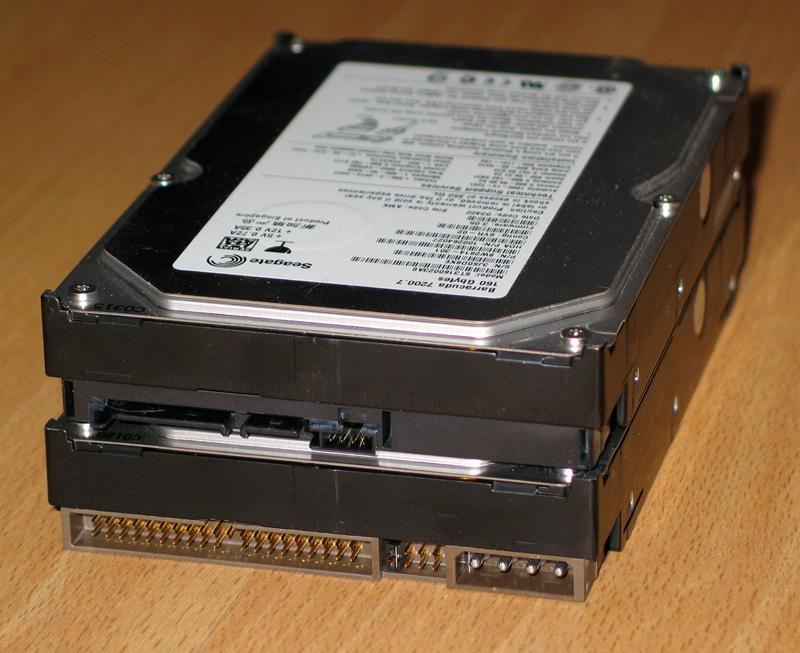
\includegraphics[scale=1.2]{pics/satavide.eps} \\
	\end{center}
\vfill


\subsection{Basic Disk Concepts: Disk Devices}
%\begin{figure}[hb]
	\begin{center}
		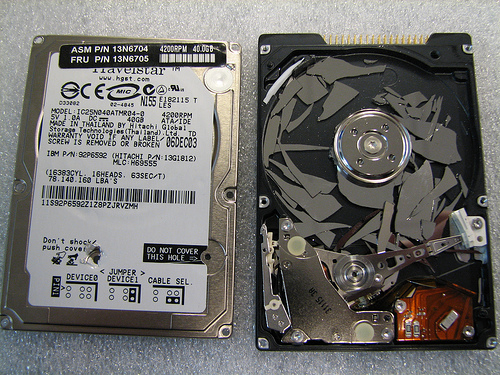
\includegraphics[scale=0.9]{pics/busted-disk.eps} \\
	\end{center}
%\end{figure}

\subsection{Basic Disk Concepts: Disk Devices}
\vfill
	\begin{center}
		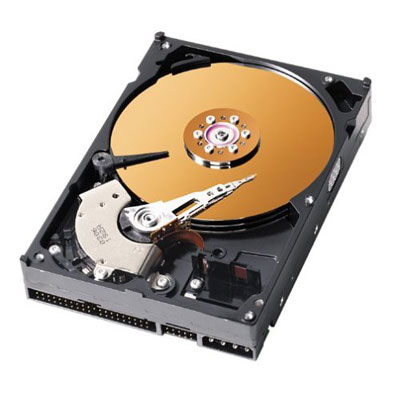
\includegraphics[scale=1.2]{pics/hard-drive.eps} \\
	\end{center}
\vfill


\subsection{Basic Disk Concepts: Disk Devices}
\vfill
	\begin{center}
		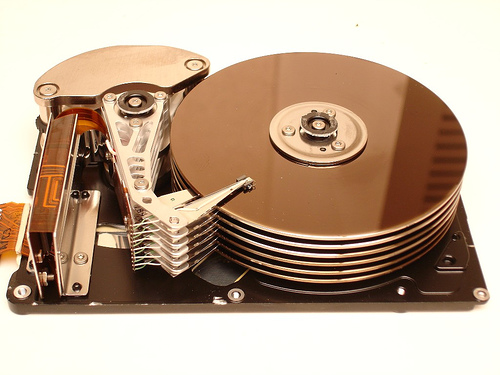
\includegraphics[scale=0.9]{pics/6platter.eps} \\
	\end{center}
\vfill

\subsection{Basic Disk Concepts: Physical Disk Structure}
\vfill
	\begin{center}
		\includegraphics[scale=1.2]{pics/cylinders.eps} \\
	\end{center}
\vfill

\subsection{Basic Disk Concepts: Physical Disk Structure}
Addressing modes:
\begin{itemize}
	\item CHS {\tt https://en.wikipedia.org/wiki/Cylinder-head-sector}
		\begin{itemize}
			\item 504 MB limitation (BIOS limited cylinders to
				1024, ATA limited heads to 16, sectors are
				limited to 6 bits (there is no sector 0))
			\item 8 GB limit (8 bits for heads)
		\end{itemize}
	\item LBA {\tt https://en.wikipedia.org/wiki/Logical\_Block\_Addressing}
		\begin{itemize}
			\item uses integer index
			\item limited to $2^{48}$ bits
		\end{itemize}
\end{itemize}

\subsection{Basic Disk Concepts: Physical Disk Structure}
Hard drive performance determined by:
\begin{itemize}
	\item seek time
	\item rotational latency
	\item internal data rate
	\item a few other negligible factors (external data rate, command
		overhead, access time, etc.)
\end{itemize}

\subsection{Basic Disk Concepts: Disk Devices}
\begin{center}
	\includegraphics[scale=2]{pics/ssd-open.eps} \\
\end{center}


\newpage
\vspace*{\fill}
\begin{center}
	\Hugesize
		Basic Disk Concepts\\ [1em]
	\hspace*{5mm}
	\blueline\\
	\hspace*{5mm}\\
		Partitions
\end{center}
\vspace*{\fill}

\subsection{Basic Disk Concepts: Partitions}
	\begin{center}
		\includegraphics[scale=1.0]{pics/disk-structure.eps} \\
		\tiny Source: SGI Techpubs \\
	\end{center}

\subsection{Basic Disk Concepts: Partitions}
	\begin{center}
		\includegraphics[scale=0.7]{pics/disk.partition.eps}
	\end{center}


\subsection{Basic Disk Concepts: Partitions}
	\begin{center}
		\includegraphics[scale=0.9]{pics/partition.eps} \\
		\tiny Source: NetBSD Guide \\
	\end{center}

\subsection{Basic Disk Concepts: Partitions}
NetBSD example (from {\tt disklabel(8)})

\begin{tabular}{ l l c }
Partition 'a': & / & \\
Partition 'b': & swap & \\
Partition 'e': & /home & \\
\end{tabular}

\begin{verbatim}
#        size    offset   fstype [fsize bsize cpg/sgs]
a:  20972385        63   4.2BSD   4096 32768  1180  # (Cyl.      0*- 20805)
b:   1048320  20972448     swap                     # (Cyl.  20806 - 21845)
c:  78140097        63   unused      0     0        # (Cyl.      0*- 77519)
d:  78140160         0   unused      0     0        # (Cyl.      0 - 77519)
e:  56119392  22020768   4.2BSD   4096 32768 58528  # (Cyl.  21846 - 77519)
\end{verbatim}

\subsection{Basic Disk Concepts: Partitions}
NetBSD example (from {\tt disklabel(8)})

\begin{tabular}{ l l c }
Partition 'a': & / & 10 GB\\
Partition 'b': & swap & \\
Partition 'e': & /home & 26 GB\\
\end{tabular}

\begin{verbatim}
#        size    offset   fstype [fsize bsize cpg/sgs]
a:  20972385        63   4.2BSD   4096 32768  1180  # (Cyl.      0*- 20805)
b:   1048320  20972448     swap                     # (Cyl.  20806 - 21845)
c:  78140097        63   unused      0     0        # (Cyl.      0*- 77519)
d:  78140160         0   unused      0     0        # (Cyl.      0 - 77519)
e:  56119392  22020768   4.2BSD   4096 32768 58528  # (Cyl.  21846 - 77519)
\end{verbatim}


\subsection{Basic Disk Concepts: Partitions}
IRIX example (from {\tt fx(1M)})

A 8.5 GB disk, with 512 MB swap:
\begin{verbatim}
part  type        blocks            Megabytes   (base+size)
  0: xfs        4096 + 16730568       2 + 8169
  1: raw    16734664 + 1048576     8171 + 512
  8: volhdr        0 + 4096           0 + 2
 10: volume        0 + 17783240       0 + 8683
----- bootinfo-----
 root partition = 0     swap partition = 1    bootfile = /unix
----- directory entries-----
  0: sgilabel   block    2 size     512  1: sash   block  3 size  266240
\end{verbatim}

\subsection{Basic Disk Concepts: Partitions}
Solaris example (from {\tt format(1m)}):
\begin{verbatim}
Current partition table (original):
Total disk cylinders available: 38758 + 2 (reserved cylinders)

Part      Tag    Flag     Cylinders         Size            Blocks
  0       root    wm       3 -  3764        3.62GB    (3762/0/0)   7584192
  1       swap    wu    3765 -  4364      590.62MB    (600/0/0)    1209600
  2     backup    wm       0 - 38757       37.26GB    (38758/0/0) 78136128
  3 unassigned    wm       0                0         (0/0/0)            0
  4 unassigned    wm       0                0         (0/0/0)            0
  5 unassigned    wm       0                0         (0/0/0)            0
  6 unassigned    wm       0                0         (0/0/0)            0
  7       home    wm    4365 - 38757       33.06GB    (34393/0/0) 69336288
  8       boot    wu       0 -     0        0.98MB    (1/0/0)         2016
  9 alternates    wu       1 -     2        1.97MB    (2/0/0)         4032
\end{verbatim}

\subsection{Basic Disk Concepts: Partitions}
Linux example (from {\tt fdisk(8)}):
\begin{verbatim}
Disk /dev/sda: 80.0 GB, 80000000000 bytes
255 heads, 63 sectors/track, 9726 cylinders
Units = cylinders of 16065 * 512 = 8225280 bytes

   Device Boot      Start         End      Blocks   Id  System
/dev/sda1   *           1          33      265041   83  Linux
/dev/sda2              34        9726    77859022+  83  Linux
\end{verbatim}

\subsection{Basic Disk and Filesystem Concepts: RAID and Logical Volumes}
Logical Volumes:
\begin{itemize}
	\item allow file systems to be larger than the physical size of a disk
	\item inrease I/O performance when {\em striped}
	\item fault tolerant when {\em mirrored} or {\em plexed}
\end{itemize}

RAID:
\begin{itemize}
	\item basic techniques:
		\begin{itemize}
			\item striping
			\item mirroring
			\item parity
		\end{itemize}
	\item different RAID levels:
		\begin{itemize}
			\item level 0 - 6
			\item level 0+1
			\item level 10, 30 or 50 (1+0, 3+0, 5+0)
		\end{itemize}
\end{itemize}

\subsection{Basic Disk and Filesystem Concepts: RAID and Logical Volumes}
\vfill
\begin{center}
	\includegraphics[scale=0.7]{pics/raid-0.eps}
	\hspace{.5in}
	\includegraphics[scale=0.7]{pics/raid-1.eps} \\
	\vspace{.2in}
	\includegraphics[scale=0.7]{pics/raid-5.eps}
\end{center}
\vfill

\subsection{Basic Disk and Filesystem Concepts: RAID and Logical Volumes}
\vfill
\begin{center}
	\includegraphics[scale=0.9]{pics/zfs.eps} \\
\end{center}
\vfill



%\subsection{Basic Disk Concepts: RAID}
%\begin{figure}[hb]
%	\begin{center}
%		\includegraphics[scale=1.1]{pics/RAID-0.eps} \\
%	\end{center}
%\end{figure}
%
%\subsection{Basic Disk Concepts: RAID}
%\begin{figure}[hb]
%	\begin{center}
%		\includegraphics[scale=1.1]{pics/RAID-1.eps} \\
%	\end{center}
%\end{figure}
%
%%\subsection{Basic Disk Concepts: RAID}
%%\begin{figure}[hb]
%%\begin{center}
%%\includegraphics[scale=1.1]{pics/RAID-2.eps} \\
%%\end{center}
%%\end{figure}
%
%\subsection{Basic Disk Concepts: RAID}
%\begin{figure}[hb]
%	\begin{center}
%		\includegraphics[scale=1.1]{pics/RAID-3.eps} \\
%	\end{center}
%\end{figure}
%
%%\subsection{Basic Disk Concepts: RAID}
%%\begin{figure}[hb]
%%	\begin{center}
%%		\includegraphics[scale=1.1]{pics/RAID-4.eps} \\
%%	\end{center}
%%\end{figure}
%
%\subsection{Basic Disk Concepts: RAID}
%\begin{figure}[hb]
%	\begin{center}
%		\includegraphics[scale=1.1]{pics/RAID-5.eps} \\
%	\end{center}
%\end{figure}
%
%%\subsection{Basic Disk Concepts: RAID}
%%\begin{figure}[hb]
%%	\begin{center}
%%		\includegraphics[scale=1.1]{pics/RAID-6.eps} \\
%%	\end{center}
%%\end{figure}
%%
%%\subsection{Basic Disk Concepts: RAID}
%%\begin{figure}[hb]
%%	\begin{center}
%%		\includegraphics[scale=1.1]{pics/RAID-7.eps} \\
%%	\end{center}
%%\end{figure}
%
%
%\subsection{Basic Disk Concepts: RAID}
%\begin{figure}[hb]
%	\begin{center}
%		\includegraphics[scale=1.1]{pics/RAID-10.eps} \\
%	\end{center}
%\end{figure}
%
%\subsection{Basic Disk Concepts: RAID}
%\begin{figure}[hb]
%	\begin{center}
%		\includegraphics[scale=1.1]{pics/RAID-0+1.eps} \\
%	\end{center}
%\end{figure}
%
%
%\subsection{Basic Disk Concepts: RAID}
%\begin{figure}[hb]
%	\begin{center}
%		\includegraphics[scale=1.1]{pics/RAID-53.eps} \\
%	\end{center}
%\end{figure}

\newpage
\vspace*{\fill}
\begin{center}
    \Hugesize
        Hooray! \\ [1em]
    \hspace*{5mm}
    \blueline\\
    \hspace*{5mm}\\
        5 Minute Break
\end{center}
\vspace*{\fill}

\newpage
\vspace*{\fill}
\begin{center}
	\Hugesize
		Basic Filesystem Concepts\\ [1em]
	\hspace*{5mm}
	\blueline\\
	\hspace*{5mm}\\
		Filesystem Layout
\end{center}
\vspace*{\fill}

\subsection{Basic Filesystem Concepts}
All partitions -- with the exception of the {\em root} (or \verb+/+) partition
-- can be {\em mounted} anywhere in the filesystem hierarchy.
\\

\begin{center}
	\includegraphics[scale=0.5]{pics/filesystem-tree-mountpoints.eps} \\
\end{center}

%\subsection{Basic Filesystem Concepts}
%All partitions -- with the exception of the {\em root} (or \verb+/+) partition
%-- can be {\em mounted} anywhere in the filesystem hierarchy.
%\\
%
%\begin{center}
%\includegraphics[scale=0.7]{pics/fs-tree-disks.eps} \\
%\end{center}
%
\subsection{Basic Filesystem Concepts}
All partitions -- with the exception of the {\em root} (or \verb+/+) partition
-- can be {\em mounted} anywhere in the filesystem hierarchy.
\\

The file \verb+/etc/fstab+ (see fstab(5)) specifies which disks / partitions
to mount where:
\\
\begin{verbatim}
/dev/wd0a   /        ffs    rw 1 1
/dev/cgd1a  none     swap   sw 0 0
/dev/cgd0a  /home    ffs    rw 1 2
/ignoreme   /tmp     mfs    rw,-b4096,-f512,-s262144 0 0
kernfs      /kern    kernfs rw
procfs      /proc    procfs rw,noauto
ptyfs       /dev/pts ptyfs  rw 0 0
\end{verbatim}
\Normalsize

\subsection{Basic Filesystem Concepts}
All partitions -- with the exception of the {\em root} (or \verb+/+) partition
-- can be {\em mounted} anywhere in the filesystem hierarchy.
\\

The file \verb+/etc/fstab+ (see fstab(5)) specifies which disks / partitions
to mount where:
\\
\small
\begin{verbatim}
# /etc/fstab: static file system information.
#
# Use 'vol_id --uuid' to print the universally unique identifier for a
# device; this may be used with UUID= as a more robust way to name devices
# that works even if disks are added and removed. See fstab(5).
#
# <file system> <mount point>   <type>  <options>       <dump>  <pass>
proc            /proc           proc    defaults        0       0
# / was on /dev/sda2 during installation
LABEL=ROOT      /       ext3    errors=remount-ro,acl   0       1
# /boot was on /dev/sda1 during installation
LABEL=BOOT      /boot   ext3    defaults,acl            0       2
# swap was on /dev/sda5 during installation
UUID=9329ae83-289d-4c3d-8756-f707c4bbb312 none            swap    sw
0       0
/dev/scd0       /media/cdrom0   udf,iso9660 user,noauto,exec,utf8 0       0
deathstar.phy.stevens-tech.edu:/export/nfs-sw/opt    /opt            nfs ro,rsize=32768,intr,nolock  0 0
deathstar.phy.stevens-tech.edu:/export/srcit-dist    /mnt/srcit-dist  nfs ro,rsize=32768,intr,nolock  0 0
corsario.cs.stevens-tech.edu:/export/people          /mnt/legacy/people nfs rw,rsize=32768,wsize=32768,intr,lock   0 0
corsario.cs.stevens-tech.edu:/export/faculty         /mnt/legacy/faculty nfs rw,rsize=32768,wsize=32768,intr,lock  0 0

\end{verbatim}
\Normalsize

\subsection{Basic Filesystem Concepts}
All partitions -- with the exception of the {\em root} (or \verb+/+) partition
-- can be {\em mounted} anywhere in the filesystem hierarchy.
\\

The file \verb+/etc/fstab+ (see fstab(5)) specifies which disks / partitions
to mount where:
\\
\small
\begin{verbatim}
#device         device          mount           FS      fsck    mount   mount
#to mount       to fsck         point           type    pass    at boot options
#
fd              -               /dev/fd         fd      -       no      -
/proc           -               /proc           proc    -       no      -
/dev/dsk/c0d0s1 -               -               swap    -       no      -
/dev/dsk/c0d0s0 /dev/rdsk/c0d0s0  /             ufs     1       no      -
/dev/dsk/c0d0p0:boot  -         /boot           pcfs    -       no      -
/dev/dsk/c0d0s7 /dev/rdsk/c0d0s7  /export/home  ufs     2       yes
-
/devices        -               /devices        devfs   -       no      -
ctfs            -               /system/contract ctfs   -       no      -
objfs           -               /system/object  objfs   -       no      -
swap            -               /tmp            tmpfs   -       yes     -
\end{verbatim}
\Normalsize



\subsection{Basic Filesystem Concepts}
All partitions -- with the exception of the {\em root} (or \verb+/+) partition
-- can be {\em mounted} anywhere in the filesystem hierarchy.
\\

To see what filesystems are currently mounted, run \verb+mount(8)+:
\\

\begin{verbatim}
/dev/wd0a on / type ffs (local)
/dev/cgd0a on /home type ffs (local)
mfs:276 on /tmp type mfs (synchronous, local)
kernfs on /kern type kernfs (local)
ptyfs on /dev/pts type ptyfs (local)
\end{verbatim}


\subsection{Basic Filesystem Concepts}
\\

\small
\begin{verbatim}
$ mount
/dev/sda2 on / type ext3 (rw,errors=remount-ro,acl)
tmpfs on /lib/init/rw type tmpfs (rw,nosuid,mode=0755)
proc on /proc type proc (rw,noexec,nosuid,nodev)
sysfs on /sys type sysfs (rw,noexec,nosuid,nodev)
varrun on /var/run type tmpfs (rw,nosuid,mode=0755)
varlock on /var/lock type tmpfs (rw,noexec,nosuid,nodev,mode=1777)
udev on /dev type tmpfs (rw,mode=0755)
tmpfs on /dev/shm type tmpfs (rw,nosuid,nodev)
devpts on /dev/pts type devpts (rw,noexec,nosuid,gid=5,mode=620)
fusectl on /sys/fs/fuse/connections type fusectl (rw)
lrm on /lib/modules/2.6.28-17-generic/volatile type tmpfs (rw,mode=755)
/dev/sda1 on /boot type ext3 (rw,acl)
securityfs on /sys/kernel/security type securityfs (rw)
automount(pid2623) on /home type autofs (rw,fd=4,pgrp=2623,minproto=2,maxproto=4)
deathstar.phy.stevens-tech.edu:/export/nfs-sw/opt on /opt type nfs (ro,rsize=32768,intr,nolock,addr=155.246.89.4)
deathstar.phy.stevens-tech.edu:/export/srcit-dist on /mnt/srcit-dist type nfs (ro,rsize=32768,intr,nolock,addr=155.246.89.4)
corsario.cs.stevens-tech.edu:/export/people on /mnt/legacy/people type nfs (rw,rsize=32768,wsize=32768,intr,lock,addr=155.246.89.20)
corsario.cs.stevens-tech.edu:/export/faculty on /mnt/legacy/faculty type nfs (rw,rsize=32768,wsize=32768,intr,lock,addr=155.246.89.20)
binfmt_misc on /proc/sys/fs/binfmt_misc type binfmt_misc (rw,noexec,nosuid,nodev)
deathstar.phy.stevens-tech.edu:/export/home/kamberov on /home/kamberov type nfs (rw,sync,intr,vers=3,sloppy,addr=155.246.89.4)
deathstar.phy.stevens-tech.edu:/export/home/mweiss on /home/mweiss type nfs (rw,sync,intr,vers=3,sloppy,addr=155.246.89.4)
deathstar.phy.stevens-tech.edu:/export/home/jschauma on /home/jschauma type nfs (rw,sync,intr,vers=3,sloppy,addr=155.246.89.4)
\end{verbatim}
\Normalsize

\subsection{Basic Filesystem Concepts}
Some of the different kinds of filesystems:

\subsection{Basic Filesystem Concepts}
Some of the different kinds of filesystems:
\begin{itemize}
	\item ``Regular'' File Systems
	\item Journaling File Systems
	\item Network File Systems
	\item Various
\end{itemize}

\newpage
\vspace*{\fill}
\begin{center}
	\Hugesize
		Basic Filesystem Concepts\\ [1em]
	\hspace*{5mm}
	\blueline\\
	\hspace*{5mm}\\
		The UNIX Filesystem
\end{center}
\vspace*{\fill}

\subsection{Basic Filesystem Concepts: The UNIX Filesystem}
The filesystem is responsible for storing the data on the disk.
So to read/write data, it needs to know in which physical blocks the actual
data is located; ie how to map files to the disk blocks.


\subsection{Basic Filesystem Concepts: The UNIX Filesystem}
\vspace*{\fill}
\begin{center}
\includegraphics[scale=0.95]{pics/bucket.eps} \\
\end{center}
\vspace*{\fill}

\subsection{Basic Filesystem Concepts: The UNIX Filesystem}
\begin{center}
\includegraphics[scale=0.95]{pics/two-buckets.eps} \\
\end{center}

\subsection{Basic Filesystem Concepts: The UNIX Filesystem}
\vspace*{\fill}
\begin{center}
\includegraphics[scale=1.0]{pics/three-buckets.eps} \\
\end{center}
\vspace*{\fill}

\subsection{Basic Filesystem Concepts: The UNIX Filesystem}
\vspace*{\fill}
\begin{center}
\includegraphics[scale=0.95]{pics/buckets.eps} \\
\end{center}
\vspace*{\fill}

\subsection{Basic Filesystem Concepts: The UNIX Filesystem}
\vspace*{\fill}
\begin{center}
\includegraphics[scale=0.95]{pics/labels.eps} \\
\end{center}
\vspace*{\fill}

\subsection{Basic Filesystem Concepts: The UNIX Filesystem}
\begin{center}
\includegraphics[scale=0.95]{pics/one-bucket-full.eps} \\
\end{center}

\subsection{Basic Filesystem Concepts: The UNIX Filesystem}
\vspace*{\fill}
\begin{center}
\includegraphics[scale=0.5]{pics/one-bucket-full.eps}
\hspace*{5mm}
\includegraphics[scale=0.6]{pics/cat-in-bucket.eps}
\end{center}
\vspace*{\fill}

\subsection{Basic Filesystem Concepts: The UNIX Filesystem}
\vspace*{\fill}
\begin{center}
\includegraphics[scale=0.95]{pics/two-cats-one-bucket.eps} \\
\end{center}
\vspace*{\fill}

\subsection{Basic Filesystem Concepts: The UNIX Filesystem}
\begin{center}
\includegraphics[scale=0.8]{pics/bucket-barbies.eps} \\
\end{center}

\subsection{Basic Filesystem Concepts: The UNIX Filesystem}
\vspace*{\fill}
\begin{center}
\includegraphics[scale=0.95]{pics/bucket-full-of-stones.eps} \\
\end{center}
\vspace*{\fill}

\subsection{Basic Filesystem Concepts: The UNIX Filesystem}
\vspace*{\fill}
\begin{center}
\includegraphics[scale=1.2]{pics/bucket-fragmented.eps} \\
\end{center}
\vspace*{\fill}

\subsection{Basic Filesystem Concepts: The UNIX Filesystem}
The filesystem is responsible for storing the data on the disk.
So to read/write data, it needs to know in which physical blocks the actual
data is located; ie how to map files to the disk blocks.
\\

Components of the Berkeley Fast Filesystem:
\\

\newcolumntype{S}{>{\centering\arraybackslash} m{.4\linewidth} }
\begin{tabular}{ p{10cm} S }
\begin{itemize}
	\item set of {\em inode} storage cells
\end{itemize}
& \multirow{2}{*}{\includegraphics[scale=0.5]{pics/buckets.eps}} \\
\end{tabular}

\subsection{Basic Filesystem Concepts: The UNIX Filesystem}
The filesystem is responsible for storing the data on the disk.
So to read/write data, it needs to know in which physical blocks the actual
data is located; ie how to map files to the disk blocks.
\\

Components of the Berkeley Fast Filesystem:
\\

\begin{tabular}{ p{10cm} S }
\begin{itemize}
	\item set of {\em inode} storage cells
	\item set of scattered ``superblocks''
\end{itemize}
& \multirow{2}{*}{\includegraphics[scale=0.3]{pics/lego.eps}} \\
\end{tabular}

\subsection{Basic Filesystem Concepts: The UNIX Filesystem}
The filesystem is responsible for storing the data on the disk.
So to read/write data, it needs to know in which physical blocks the actual
data is located; ie how to map files to the disk blocks.
\\

Components of the Berkeley Fast Filesystem:
\\

\begin{tabular}{ p{10cm} S }
\begin{itemize}
	\item set of {\em inode} storage cells
	\item set of scattered ``superblocks''
	\item map of disk blocks
\end{itemize}
& \multirow{2}{*}{\includegraphics[scale=0.5]{pics/map.eps}} \\
\end{tabular}

\subsection{Basic Filesystem Concepts: The UNIX Filesystem}
The filesystem is responsible for storing the data on the disk.
So to read/write data, it needs to know in which physical blocks the actual
data is located; ie how to map files to the disk blocks.
\\

Components of the Berkeley Fast Filesystem:
\\

\begin{tabular}{ p{10cm} S }
\begin{itemize}
	\item set of {\em inode} storage cells
	\item set of scattered ``superblocks''
	\item map of disk blocks
	\item block usage summary
\end{itemize}
& \multirow{2}{*}{\includegraphics[scale=0.5]{pics/tetris.eps}} \\
\end{tabular}

\subsection{Basic Filesystem Concepts: The UNIX Filesystem}
The filesystem is responsible for storing the data on the disk.
So to read/write data, it needs to know in which physical blocks the actual
data is located; ie how to map files to the disk blocks.
\\

Components of the Berkeley Fast Filesystem:
\\

\begin{tabular}{ p{10cm} S }
\begin{itemize}
	\item set of {\em inode} storage cells
	\item set of scattered ``superblocks''
	\item map of disk blocks
	\item block usage summary
	\item set of data blocks
\end{itemize}
& \multirow{2}{*}{\includegraphics[scale=0.3]{pics/block.eps}} \\
\end{tabular}

\subsection{Basic Filesystem Concepts: The UNIX Filesystem}
\begin{center}
	\includegraphics[scale=0.8]{pics/ufs-details.eps} \\
\end{center}
\vspace*{\fill}

\subsection{Basic Filesystem Concepts: The UNIX Filesystem}
\begin{verbatim}
$ ec2-run-instances -g stevens -k stevens ami-3c47a355
$ ec2-describe-instances
$ ssh <hostname>
# mount
# cat /etc/fstab
# df
# df -i
# dumpe2fs /dev/sda1 | less
\end{verbatim}


\subsection{Basic Filesystem Concepts: The UNIX Filesystem}
Information stored in an {\em inode}:

\subsection{Basic Filesystem Concepts: The UNIX Filesystem}
Information stored in an {\em inode}:
\begin{itemize}
	\item user owner and group owner ID's
\end{itemize}

\subsection{Basic Filesystem Concepts: The UNIX Filesystem}
Information stored in an {\em inode}:
\begin{itemize}
	\item user owner and group owner ID's
	\item file type
\end{itemize}

\subsection{Basic Filesystem Concepts: The UNIX Filesystem}
Information stored in an {\em inode}:
\begin{itemize}
	\item user owner and group owner ID's
	\item file type
	\item access mode (permissions)
\end{itemize}

\subsection{Basic Filesystem Concepts: The UNIX Filesystem}
Information stored in an {\em inode}:
\begin{itemize}
	\item user owner and group owner ID's
	\item file type
	\item access mode (permissions)
	\item file access and modification time
\end{itemize}

\subsection{Basic Filesystem Concepts: The UNIX Filesystem}
Information stored in an {\em inode}:
\begin{itemize}
	\item user owner and group owner ID's
	\item file type
	\item access mode (permissions)
	\item file access and modification time
	\item file status modification time
\end{itemize}

\subsection{Basic Filesystem Concepts: The UNIX Filesystem}
Information stored in an {\em inode}:
\begin{itemize}
	\item user owner and group owner ID's
	\item file type
	\item access mode (permissions)
	\item file access and modification time
	\item file status modification time
	\item number of links to the file
\end{itemize}

\subsection{Basic Filesystem Concepts: The UNIX Filesystem}
Information stored in an {\em inode}:
\begin{itemize}
	\item user owner and group owner ID's
	\item file type
	\item access mode (permissions)
	\item file access and modification time
	\item file status modification time
	\item number of links to the file
	\item size of the file
\end{itemize}

\subsection{Basic Filesystem Concepts: The UNIX Filesystem}
Information stored in an {\em inode}:
\begin{itemize}
	\item user owner and group owner ID's
	\item file type
	\item access mode (permissions)
	\item file access and modification time
	\item file status modification time
	\item number of links to the file
	\item size of the file
	\item disk device containing this file
\end{itemize}

\subsection{Basic Filesystem Concepts: The UNIX Filesystem}
Information stored in an {\em inode}:
\begin{itemize}
	\item user owner and group owner ID's
	\item file type
	\item access mode (permissions)
	\item file access and modification time
	\item file status modification time
	\item number of links to the file
	\item size of the file
	\item disk device containing this file
\end{itemize}

\begin{verbatim}
$ stat /etc/passwd
$ ln /etc/passwd /tmp/passwd
$ stat /tmp/passwd
$ stat -L /tmp/passwd
\end{verbatim}

\subsection{Basic Filesystem Concepts: The UNIX Filesystem}
File types:
\\

\begin{tabular}{ p{10cm} S }
\begin{itemize}
	\item regular files
\end{itemize}
& \multirow{2}{*}{\includegraphics[scale=0.7]{pics/file.eps}} \\
\end{tabular}
\\

\verb+$ stat /etc/passwd+


\subsection{Basic Filesystem Concepts: The UNIX Filesystem}
File types:
\\

\begin{tabular}{ p{10cm} S }
\begin{itemize}
	\item regular files
	\item directories
\end{itemize}
& \multirow{2}{*}{\includegraphics[scale=1.5]{pics/directory.eps}} \\
\end{tabular}
\\

\verb+$ stat /+

\subsection{Basic Filesystem Concepts: The UNIX Filesystem}
File types:
\\

\begin{tabular}{ p{10cm} S }
\begin{itemize}
	\item regular files
	\item directories
	\item special files
\end{itemize}
& \multirow{2}{*}{\includegraphics[scale=1.0]{pics/devices.eps}} \\
\end{tabular}
\\

\verb+$ file /dev/* | more+

\subsection{Basic Filesystem Concepts: The UNIX Filesystem}
File types:
\\

\begin{tabular}{ p{10cm} S }
\begin{itemize}
	\item regular files
	\item directories
	\item special files
	\item links
\end{itemize}
& \multirow{2}{*}{\includegraphics[scale=0.6]{pics/link.eps}} \\
\end{tabular}
\\

\begin{verbatim}
$ touch /tmp/foo
$ ln /tmp/foo /tmp/bar
$ stat /tmp/foo /tmp/bar
$ ln -sf /tmp/foo /tmp/bar
$ stat /tmp/foo /tmp/bar
\end{verbatim}

\subsection{Basic Filesystem Concepts: The UNIX Filesystem}
File types:
\\

\begin{tabular}{ p{10cm} S }
\begin{itemize}
	\item regular files
	\item directories
	\item special files
	\item links
	\item sockets
\end{itemize}
& \multirow{2}{*}{\includegraphics[scale=0.8]{pics/socket.eps}} \\
\end{tabular}
\\

\verb+$ stat /dev/log+

\subsection{Basic Filesystem Concepts: The UNIX Filesystem}
File types:
\\

\begin{tabular}{ p{10cm} S }
\begin{itemize}
	\item regular files
	\item directories
	\item special files
	\item links
	\item sockets
	\item named pipes
\end{itemize}
& \multirow{2}{*}{\includegraphics[scale=1.0]{pics/pipe.eps}} \\
\end{tabular}
\\

\begin{verbatim}
$ mkfifo /tmp/fifo
$ cat /tmp/fifo > /tmp/out &
$ stat /tmp/fifo | tee /tmp/fifo
$ cat /tmp/out
\end{verbatim}

\subsection{HW\#1}
Setup your environment for EC2 and create an instance
\vfill
\verb+http://www.cs.stevens.edu/~jschauma/615/s13-hw1.html+
\vfill

\subsection{Reading}
\begin{itemize}
	\item \verb+http://is.gd/5mndwA+
	\item \verb+http://is.gd/ig4QP5+
	\item \verb+http://is.gd/9YeIKh+
\end{itemize}

\subsection{Reading}
Disk Interfaces:
\begin{itemize}
	\item SCSI:
		\begin{itemize}
			\item \verb+http://en.wikipedia.org/wiki/Scsi+
			\item scsi(4), scsictl(8);
		\end{itemize}
	\item ATA:
		\begin{itemize}
			\item \verb+http://www.ata-atapi.com/+
			\item \verb+http://wikipedia.org/wiki/Advanced_Technology_Attachment+
			\item \verb+http://en.wikipedia.org/wiki/Sata+
		\end{itemize}
	\item USB:
		\begin{itemize}
			\item \verb+http://en.wikipedia.org/wiki/Usb+
			\item \verb+http://www.usb.org/+
			\item usb(4)
		\end{itemize}
\end{itemize}

\subsection{Reading}
Disk Interfaces:
\begin{itemize}
	\item FireWire:
		\begin{itemize}
			\item \verb+http://www.apple.com/firewire/+
			\item \verb+http://en.wikipedia.org/wiki/Firewire+
		\end{itemize}
	\item Serial attached SCSI:
		\begin{itemize}
			\item \verb+https://en.wikipedia.org/wiki/Serial_attached_SCSI+
		\end{itemize}
	\item Fibre Channel:
		\begin{itemize}
			\item \verb+http://hsi.web.cern.ch/HSI/fcs/fcs.html+
			\item \verb+http://en.wikipedia.org/wiki/Fibrechannel+
		\end{itemize}
	\item AoE, FCoE, iSCSI:
		\begin{itemize}
			\item \verb+http://en.wikipedia.org/wiki/ATA_over_Ethernet+
			\item \verb+http://en.wikipedia.org/wiki/FCoE+
			\item \verb+http://en.wikipedia.org/wiki/ISCSI+
		\end{itemize}
\end{itemize}

\subsection{Reading}
Basic Disk Concepts:
\begin{itemize}
	\item \verb+http://is.gd/3SXn5N+
	\item disklabel(8), fdisk(8)
	\item format(1m)
\end{itemize}
RAID:
\begin{itemize}
	\item \verb+http://en.wikipedia.org/wiki/RAID+
\end{itemize}
Basic Filesystem Concepts:
\begin{itemize}
	\item \verb+http://is.gd/Ha8QLW+
	\item \verb+http://is.gd/YMm3JL+
	\item newfs(8)
\end{itemize}
NFS: \verb+http://www.cis.udel.edu/~srisatha/NFS/sld001.htm+

\end{document}
